\documentclass[notes,10pt, aspectratio=169]{beamer}


\usepackage{pgfpages}
% These slides also contain speaker notes. You can print just the slides,
% just the notes, or both, depending on the setting below. Comment out the want
% you want.
\setbeameroption{hide notes} % Only slide
%\setbeameroption{show only notes} % Only notes
% \setbeameroption{show notes on second screen=right} % Both

\usepackage{import}
% \usepackage{helvet} %? to change the font to Helvetica
% \usepackage[default]{lato}
% \usepackage{verbatim}

\usepackage{array}
% \usepackage{natbib}
% \bibliographystyle{plain}
\usepackage{apalike}
\bibliographystyle{apalike}
% \usepackage[natbib, maxcitenames=3, mincitenames=11, style=apa]{biblatex}

% \usepackage{fontspec} %! error

% \usefonttheme{professionalfonts} % using non standard fonts for beamer
% \usefonttheme{serif} % default family is serif

% \setmainfont{Liberation Serif}

% \setsansfont{Liberation Serif}


\usepackage{tikz}
\newcommand*\circled[4]{\tikz[baseline=(char.base)]{
 \node[shape=circle, fill=#2, draw=#3, text=#4, inner sep=2pt] (char) {#1};}}



\setbeamertemplate{note page}{\pagecolor{yellow!5}\insertnote}
\usetikzlibrary{positioning}
\usetikzlibrary{snakes}
\usetikzlibrary{calc}
\usetikzlibrary{arrows}
\usetikzlibrary{decorations.markings}
\usetikzlibrary{shapes.misc}
\usetikzlibrary{matrix,shapes,arrows,fit,tikzmark}
\usepackage{amsmath}
\usepackage{mathpazo}
\usepackage{hyperref}
\usepackage{lipsum}
\usepackage{multimedia}
\usepackage{graphicx}
\usepackage{multirow}
\usepackage{graphicx}
\usepackage{dcolumn}
\usepackage{bbm}
\usepackage{cancel}
\newcolumntype{d}[0]{D{.}{.}{5}}
\usepackage{subcaption}
\usepackage{changepage}
\usepackage{appendixnumberbeamer}
\newcommand{\beginbackup}{
 \newcounter{framenumbervorappendix}
 \setcounter{framenumbervorappendix}{\value{framenumber}}
 \setbeamertemplate{footline}
 {
 \leavevmode%
 \hline
 box{%
 \begin{beamercolorbox}[wd=\paperwidth,ht=2.25ex,dp=1ex,right]{footlinecolor}%
% \insertframenumber \hspace*{2ex} 
 \end{beamercolorbox}}%
 \vskip0pt%
 }
 }
\newcommand{\backupend}{
 \addtocounter{framenumbervorappendix}{-\value{framenumber}}
 \addtocounter{framenumber}{\value{framenumbervorappendix}} 
}


\usepackage{graphicx}
\usepackage[space]{grffile}
\usepackage{booktabs}

% These are my colors -- there are many like them, but these are mine.
\definecolor{blue}{RGB}{70,160,205}
\definecolor{red}{RGB}{213,94,0}
\definecolor{yellow}{RGB}{240,228,66}
\definecolor{green}{RGB}{0,158,115}

% % Enviroments
% \newtheorem{defin}{Definition.}
% \newtheorem{teo}{Theorem. }
% \newtheorem{lema}{Lemma. }
% \newtheorem{coro}{C
% \begin{frame}{Modeling Choice}orolary. }
% \newtheorem{prop}{Proposition. }
% \theoremstyle{definition}
% \newtheorem{examp}{Example. }
% % \numberwithin{problem}{subsection} 

\hypersetup{
 colorlinks=false,
 linkbordercolor = {white},
 linkcolor = {blue} 
}

\newcommand\Fontvi{\fontsize{8.5}{7.2}\selectfont}

\newcommand\Fontx{\fontsize{10}{7.2}\selectfont}
%% I use a beige off-white for my background
\definecolor{MyBackground}{RGB}{255,253,218}

%% Uncomment this if you want to change the background color to something else
%\setbeamercolor{background canvas}{bg=MyBackground}

%% Change the bg color to adjust your transition slide background color!
\newenvironment{transitionframe}{
 \setbeamercolor{background canvas}{bg=white}
 \begin{frame}}{
 \end{frame}
}

\setbeamercolor{frametitle}{fg=blue}
\setbeamercolor{title}{fg=black}
\setbeamertemplate{footline}[frame number]
\setbeamertemplate{navigation symbols}{} 
\setbeamertemplate{itemize items}{-}
% \setbeamertemplate{itemize items}[circle]   
% \setbeamertemplate{itemize subitem}[triangle]
% \setbeamertemplate{itemize subsubitem}[circle]
% \setbeamertemplate{enumerate items}[default]
% \setbeamertemplate{section in toc}[circle]
% \setbeamertemplate{subsection in toc}[triangle]
% \setbeamertemplate{subsubsection in toc}[square]


\setbeamercolor{itemize item}{fg=blue}
\setbeamercolor{itemize subitem}{fg=blue}
\setbeamercolor{itemize subsubitem}{fg=blue}
\setbeamercolor{enumerate item}{fg=blue}
\setbeamercolor{enumerate subitem}{fg=blue}
\setbeamercolor{enumerate subsubitem}{fg=blue}
\setbeamercolor{button}{bg=MyBackground,fg=blue,}
\setbeamercolor{theotem}{fg=blue} 

% If you like road maps, rather than having clutter at the top, have a roadmap show up at the end of each section 
% (and after your introduction)
% Uncomment this is if you want the roadmap!
%\AtBeginSection[]
%{
% \begin{frame}
% \frametitle{Roadmap of Talk}
% \tableofcontents[currentsection]
% \end{frame}
%}

%  buttons transparent:
% \setbeamertemplate{button}{\tikz
%  \node[
%  inner xsep=10pt,
%  draw=structure!80,
%  fill=structure!50,
%  rounded corners=4pt]  {\insertbuttontext};}

\setbeamercolor{section in toc}{fg=blue}
\setbeamercolor{subsection in toc}{fg=red}
\setbeamersize{text margin left=1em,text margin right=1em} 

\newenvironment{wideitemize}{\itemize\addtolength{\itemsep}{10pt}}{\enditemize}

\usepackage{environ}
\NewEnviron{videoframe}[1]{
 \begin{frame}
 \vspace{-8pt}
 \begin{columns}[onlytextwidth, T] % align columns
 \begin{column}{.58\textwidth}
 \begin{minipage}[t][\textheight][t]
 {\dimexpr\textwidth}
 \vspace{8pt}
 \hspace{4pt} {\Large \sc \textcolor{blue}{#1}}
 \vspace{8pt}
 
 \BODY
 \end{minipage}
 \end{column}%
 \hfill%
 \begin{colußmn}{.42\textwidth}
 \colorbox{green!20}{\begin{minipage}[t][1.2\textheight][t]
 {\dimexpr\textwidth}
 Face goes here
 \end{minipage}}
 \end{column}%
 \end{columns}
 \end{frame}
}
% * Changing Font



% Unraveling Deposit Dynamics: Local Bank Competition and Segmented Deposit Markets

\title[]{\textcolor{blue}{The Deposit Business at Large vs. Small Banks}} %, Rate Dispersion and Profits in 

\subtitle{\textcolor{blue}{Adrien d'Avernas, Andrea L. Eisfeldt,Can Huang,Richard Stanton,Nancy Wallace}}
\author{Presenter: Giselle Labrador-Badia}
% university
\institute{University of Wisconsin-Madison}
%\centering
\date{\today}


\begin{document}
%%% TIKZ STUFF
\tikzset{ 
 every picture/.style={remember picture,baseline},
 every node/.style={anchor=base,align=center,outer sep=1.5pt},
 every path/.style={thick},
 }
\newcommand\marktopleft[1]{%
 \tikz[overlay,remember picture] 
 \node (marker-#1-a) at (-.3em,.3em) {};%
}
\newcommand\markbottomright[2]{%
 \tikz[overlay,remember picture] 
 \node (marker-#1-b) at (0em,0em) {};%
}
\tikzstyle{every picture}+=[remember picture] 
\tikzstyle{mybox} =[draw=black, very thick, rectangle, inner sep=10pt, inner ysep=20pt]
\tikzstyle{fancytitle} =[draw=black,fill=red, text=white]
%%%% END TIKZ STUFF

% % Title Slide
\begin{frame}[noframenumbering]
 \maketitle
\end{frame}



% \begin{frame}{Introduction}

%     \vspace{0.2cm}

%     \begin{wideitemize}
%         % \item Deregulation story: short until Riegle Act
%         \item %\textcolor{blue}{Background:}
%  Digital banking platforms have become widespread as an alternative to traditional physical branches.
%         \item Effects on competition are unclear: 
        
%         \vspace{0.2cm}
%         \begin{wideitemize}
%             \item size distributions of banks (scale economies, lower investment costs),
%             \item banking products (loans, deposits).

%         \end{wideitemize}
%         \item Competition $\rightarrow$ stability.
%         \pause
%         \item \textcolor{blue}{How does the digital revolution affect competition and stability?} 

%         % \item \textcolor{blue}{Preview of results}:
%             \vspace{0.2cm}
%             \begin{wideitemize}
%                 \vspace{0.2cm}
%                 \item  $\uparrow$ competition, $\downarrow$ stability.

%             \end{wideitemize}

%         % \item 

%     \end{wideitemize}
%     % \item Banks compete for deposits

% \end{frame}

% \begin{frame}{Introduction}

%     \begin{wideitemize}
      
%         \item \textcolor{blue}{Preview of results}:

%     % \item \textcolor{blue}{Preview of results}:
%         \vspace{0.2cm}
%         \begin{wideitemize}
%             \vspace{0.2cm}
%             \item  $\uparrow$ competition, $\downarrow$ stability.
%             \item After digitalization:
%             \vspace{0.2cm}
%             \begin{itemize} 
%                 \item banks operate in more markets, and mid-size banks grow faster.
%             \item More uninsured deposits in balance sheets, and more loans to high-income borrowers.
%             \end{itemize}
%             \item Structural model of the U.S. banking industry to compare counterfactual without digitalization.

%             % \item Provide a theory that rationalizes the observed patterns (framework Oberfield et al. (2024)).
%             \begin{itemize}
%                 \vspace{0.2cm}
%                 \item $\uparrow$ competition, $\downarrow$ stability.
%                 \item $\uparrow$ consumer surplus and banks profits. 

%             \end{itemize}

%         \end{wideitemize}


%     \end{wideitemize}
% \end{frame}

% \begin{frame}{Introduction}

%     \begin{wideitemize}
        
%         \item \textcolor{blue}{Contribution:} 
%                 \vspace{0.2cm}
%         \begin{wideitemize}
%             \item How digital platforms alter competition in banking. \footnote{Dreschsler et al. (2017), Honka et al. (2014), Hatfield and Wallen (2022), Vives and Ye (2022), Jiant et al. (2020)}
    
%             \item Effects on banks' screening and monitoring abilities by finding greater per-unit loan losses and more loans to high-income borrowers.
%             \footnote{Fishman et al. (2017), Stein (2022), and Gornall et al. (2023), Di Maggio and Yao (2021), Liberti and Petersen (2019)}
            
%             \item Effect on digital platforms on banks' funding composition and stability. \footnote{Diamond and Dybvig (1983), Egan et al. (2019), Jiang et al. (2023), Drechler et al. (2023), Benmelech et al. (2023).}
        
%             \item Banks technology adoption by endogenizing digital platform adoption. \footnote{Vives (2019), Jiang et al. (2022), Haendler (2022).}
            

%         \end{wideitemize}
%         % \item Banks compete for deposits
%     \end{wideitemize}
    
% \end{frame}
    
% Slide 1: Motivation and Research Questions
\begin{frame}{Motivation and Research Questions}
    \begin{wideitemize}
        \item Large and small banks differ significantly in how they operate their deposit franchises.
        \item These differences impact deposit rates, rate elasticities, customer bases, and market strategies.
        \item \textcolor{blue}{Main Goals/Questions:}
        \vspace{0.2cm}
        \begin{wideitemize}
            % \item Why do large banks offer uniform deposit rates and lower rates than small banks?
            \item How do differences in preferences and technologies drive this behavior, rather than market power?
            \item What are the implications for financial stability and bank valuation?
        \end{wideitemize}
        \item \textcolor{blue}{Trade-offs:}
        \vspace{0.2cm}
        \begin{wideitemize}
            \item Large banks face higher fixed costs for superior service but use uniform pricing.
            \item Small banks offer higher rates but face higher rate sensitivities and lower service quality.
        \end{wideitemize}
    \end{wideitemize}
    \end{frame}
    
    % Slide 2: Preview of Results and Contributions
    \begin{frame}{Preview of Results and Contributions}
    \begin{wideitemize}
        \item Large banks operate in high-income, densely populated markets with less rate-elastic customers.
        \item Small banks offer higher deposit rates, especially where large banks are absent.
        \item Empirical evidence supports that uniform pricing by large banks is driven by technology and customer preferences.
        \item Structural model links bank size, pricing strategies, and market location decisions.
        \item Provides insights into deposit franchises’ role in bank valuations and financial stability.
    \end{wideitemize}
    \end{frame}
    
    % Slide 3: Literature Connections
    \begin{frame}{Literature}
    \begin{wideitemize}
        \item Deposit pricing and competition \footnote{ Drechsler et al. (2017, 2021), Jiang et al. (2023),Egan et al. (2017), Xiao (2020),
        Granja and Paxiao (2024).}
        \item Bank valuation and deposit franchises \footnote{Minton et al. (2019), Egan et al. (2022)}
        \item Bank industry equilibrium models \footnote{Corbae and D’Erasmo (2021, 2013), Wang et al. (2022).}
        \item Technology adoption and services \footnote{Haendler (2023), Sarkisyan (2023).}

    \end{wideitemize}
    \end{frame}
    
    
% ********************************************************************************************************************


\begin{frame}[noframenumbering]

    \huge \centering \textcolor{blue}{Model}
    % \\
    % \centering \textcolor{blue}{Banking for large and small banks}
    
    \end{frame}


    \begin{frame}{ Demand for banking services}
    
        \begin{wideitemize}

            \item $k \in \{1, ..., K\}$ local markets with mass of $M_k$ depositors.
            
            \item Each depositors is endowed with one dollar.
    
            \item Depositor $i$ in $k$ and maximize utility:
            
            \begin{equation}
            \max _{j \in \mathcal{B}_k} \quad \mu_{i b}=\alpha_{k} (r_j - r_f) + \beta_k x_j + \epsilon_{ijk} = - \alpha_{k} s_j + \beta_k x_j + \epsilon_{ijk}
            \end{equation}
    
            \begin{itemize}
                \item $r_j$ is the deposit interest rate on bank $j$ (uniform), 
                \item $r_f$ is the competitive risk-free rate,
                \item $x_j$ are bank characteristics,
                \item $\epsilon_{ijk}$ is the idiosyncratic taste for bank $j$ that distributes as a T1EV.
            \end{itemize}
  
            \item Total demand is $D_{jk} = M_k d_{jk}$.
            Market share of bank $j$ in $k$ is: 
            $$ 
            d_{jk} = \frac{\exp (-\alpha_k s_j + \beta_k x_j)}{1 + \sum_{j' \in \mathcal{B}_k} \exp (-\alpha_k s_{j'} + \beta_k x_{j'})}
            $$
        \end{wideitemize}
    
    
        \end{frame}

            \begin{frame}{Banks}
            
                \begin{wideitemize}
                \item Bank $j$'s problem is: 
                \begin{equation}
                \begin{aligned}
                    \max _{x_j, b_{jk},s_j} & \quad \sum_{k\in\mathcal{M}_j}^K ((s_j-c)D_{jk} - \kappa_k)b_{jk} - \chi x_j  \\
                    \end{aligned}
                \end{equation}

                \begin{itemize}
                    \item $b_{jk}=1$ if the banks decides to operate in $k$,
                    \item $c$ is the variable costs of servicing deposits (marginal?),
                    \item $\kappa$ is the cost of opening a branch in $k$,
                    \item $\chi$ is the cost of of additional funancial services $x_j \in \{0,1\}$, and,
                    \item $\mathcal{M}_j$ is the set of markets in which bank $j$ operates ($k: b_{jk}=1$).
                \end{itemize}
                \item The deposit rate that maximizes profits is:
                    \begin{equation}
                        \begin{align}
                    \sum_{k\in\mathcal{M}_j}^K D_{jk} + (s_j-c)   \sum_{k\in\mathcal{M}_j}^K \frac{\partial D_{jk}}{\partial s_j} &= 0 \\
                    s_j = c -(\eta_j^s)^{-1} 
                    \end{align}
                    \end{equation}

                \item where $\eta_j^s$ is the weighted semielasticity of demand for bank $j$, $\eta_j^s = \sum_{k\in\mathcal{M}_j}^K \frac{\alpha_k D_{jk} (1-d_{jk})}{\sum_{k\in\mathcal{M}_j}^K D_{jk}}$.
                    \end{wideitemize}
                
            \end{frame}
            
            
            \begin{frame}{Model implications}
            
                \begin{wideitemize}
                    \item \textcolor{blue}{Assumption:} $b_{jk} = 1$ if and only if $(s_j -c)D_{jk} >\kappa $.
                    \item Entry in a market means acquiring an existing branch at market value $\kappa$.
                    \item \textcolor{blue}{Equilibrium}: Given the parameters $\theta = \{\alpha_k, \beta_k, c, \kappa, \chi, M_k\}_{k=1}^K$, the equilibrium is a set of choices $j_{ik}^*$, $b_{jk}^*$, $x_j$ and $s_j^*$ such that it solves (1) and (2) for all $i$, $j$ and $k$, market clears and free entry holds.
                    \item \textcolor{blue}{Proposition 1. (Free-entry condition)} 
                    The free-entry condition in market $k$ is such that the number of single-market banks (suprascript $S$) entering market $k$ is given by
                    $$
                    N_k^S=\left\lfloor\frac{M_k}{\kappa_k \alpha_k}-\Omega_k e^{\alpha_k s_k^S-\beta_k x_k^S}+1\right\rfloor\left(\quad \text { if } \quad N_k^S>0\right.
                    $$
                    where $\theta_k \in[0,1), \Omega_k=\sum_{i \in \mathcal{ L}_k} \exp \left(-\alpha_k s_i+\beta_k x_i\right)$, and $\mathcal{L}_k \equiv\left\{j: b_{j k}=1\right.$ and $\left.\left|\mathcal{M}_j\right|>1\right\}$ is the set of multi-market banks entering market $k$.


                \end{wideitemize}
                
                
            
            \end{frame}
            % Proposition 2 derives an equilbrium result with two types of banks. We have large banks $(L)$ that invest in financial services and operate across various markets by opening multiple branches, and small banks $(S)$ that do not invest in financial services and only open a branch in a single market. We use the superscript $S$ or $L$ to denote choice variables pertaining to small or large banks, respectively.

% Proposition 2 (Small banks operate in one market). If $x_j=0$, then $\left|\mathcal{M}_j\right|=1$.
% These results highlight the trade-off between bearing the cost of financial-service technologies, which is profitable only when operating at a large scale across multiple markets, and the capacity of small banks to set rates fine-tuned to individual markets. In other words, a bank constrained to set a deposit spread different from the optimal spread in a given market cannot compete with other unrestricted single-branch banks, unless it also offers additional financial services. ${ }^{14}$ 
%             As we demonstrate below, the model ofers strong predictions regarding the disparity
% between markets where large banks operate and markets with only small banks. For these
% propositions, we defne collocation markets to be the set of markets C where both small and
% large banks operate, C = {k : ∃j, bjk = 1 and |Mj > 1|}. Proposition 3 provides a condition
% for such markets.
% Proposition 3 (Collocation markets’ demand). If i ∈ C, the ratio of deposits supplied by
% small and large banks is given by
% ! Dk
% S
% � L S log = α s − s − βk. (13) j k DL
% jk
% Proposition 3 illustrates that in collocation markets, small banks engage in competition
% for deposits by ofering lower deposit spreads, while large banks beneft from the preference
% for fnancial services βk.

% Proposition 4 (Deposit spreads and average spread semi-elasticity). Given (7), si < sj if
%                 and only if |ηs| > |ηs|.
            
            \begin{frame}{Model implications}
            
            \begin{wideitemize}

                \item \textit{Large banks}, $L$, operate in multiple markets and invest in financial services.
                
                \item \textit{Small banks}, $S$, operate in one market and do not invest in financial services.
                
                \item  \textcolor{blue}{Proposition 2. (Small banks operate in one market)}   If $x_j=0$, then $\left|\mathcal{M}_j\right|=1$.
                \item \textcolor{blue}{Collocation markets’ demand}  If $i \in C$, the ratio of deposits supplied by small and large banks is given by
                $$ \frac{D_{jk}^S}{D_{jk}^L} = \exp(\alpha_k s^L - s^S - \beta_k)$$
                where $C = \{k: \exists j, b_{jk}=1 \text{ and } |\mathcal{M}_j|>1\}$.

                \item  \textcolor{blue}{Proposition 4. (Deposit spreads and average spread semi-elasticity)} $s_i < s_j$ if and only if $|\eta_i^s| > |\eta_j^s|$.
            \end{wideitemize}
            \end{frame}
            
%             Proposition 5 (Large banks' location). If

% $$
% \frac{\alpha_k}{\left|\eta_j^s\right|}-\log \left(\frac{\alpha_k}{\left|\eta_j^s\right|}\right) \beta 1+\beta_k x_j+\frac{\kappa_k \alpha_k}{M_k}
% $$

% then bank $j$ does not locate in market $k$.
% Given a distribution of $\alpha_k$ 's, large banks maximize their profits by choosing a deposit spread that allows them to open branches in the largest possible number of markets. If the distribution is heavily skewed, we would therefore expect large banks to locate in markets close to the median, and neglect markets with large sensitivities to deposit rates.

% Proposition 6 demonstrates that if we observe two markets-one where a large bank locates and another where it does not locate - then the latter market must have a rate sensitivity that is further away from its semi-elasticity $\eta^s$.
% Proposition 6 (Collocation markets). Assume that $M_k / \kappa_k \geq M_{\ell} / \kappa_{\ell}$ and $\beta_k \leq \beta_{\ell}$. If $k \in \mathcal{M}_j$ and $\ell \notin \mathcal{M}_j$, then

% $$
% \frac{\alpha_k}{\left|\eta_j^s\right|}-\log \left(\frac{\alpha_k}{\left|\eta_j^s\right|}\right)\left(<\frac{\alpha_{\ell}}{\left|\eta_j^s\right|}-\log \left(\frac{\alpha_{\ell}}{\left|\eta_j^s\right|}\right)(\right.
% $$


% Proposition 7 demonstrates how heterogeneity in market competition differs whether the heterogeneity is driven by difference in entry costs or the rate sensitivities. For simplicity, consider a market with only small banks. If the cost of opening a branch $\kappa_k$ increases, then net profits decrease, fewer banks enter, and competition, measured by deposit spreads or the

\begin{frame}{Model implications}
            
    \begin{wideitemize}

        \item \textcolor{blue}{Proposition 5. (Large banks' location)} Bank $j$ does not locate in market $k$ if
        $$
        \frac{\alpha_k}{\left|\eta_j^s\right|}-\log \left(\frac{\alpha_k}{\left|\eta_j^s\right|}\right) \beta 1+\beta_k x_j+\frac{\kappa_k \alpha_k}{M_k}
        $$
        \item \textcolor{blue}{Proposition 6. (Collocation markets)} If $k \in \mathcal{M}_j$ and $\ell \notin \mathcal{M}_j$, then 
        $$
        \frac{\alpha_k}{\left|\eta_j^s\right|}-\log \left(\frac{\alpha_k}{\left|\eta_j^s\right|}\right)<\frac{\alpha_{\ell}}{\left|\eta_j^s\right|}-\log \left(\frac{\alpha_{\ell}}{\left|\eta_j^s\right|}\right)
        $$
    \end{wideitemize}
    \end{frame}
    % have that net profits decrease and fewer banks enter. However competition, as measured by deposit spreads, improves! From the perspective of a bank, a market with higher rate semi-elasticity is a more competitive environment, while a market with a higher entry cost is less competitive. However, HHI only depends on the number of banks, which decreases in both cases. In the next section, we find that $\alpha_k$ explains more variation in deposit spreads than HHI.

    % Proposition 7 (Herfindahl-Hirschman index). If $k \notin \mathcal{C}$, then
    
    % $$
    % d_k^S=\frac{1}{1+\frac{M_k}{\kappa_k \alpha_k}}, \quad s_k^S=c+\frac{1}{\alpha_k}+\frac{\kappa_k}{M_k}, \quad \text { and } H H I_k=\frac{10000}{1+\frac{M_k}{\kappa_k \alpha_k}} .
    % $$
    
    
    % Thus,
    
    % $$
    % \frac{\partial s_k^S}{\partial \alpha_k} \frac{\partial \alpha_k}{\partial H H I_k}<0 \text { and } \frac{\partial s_k^S}{\partial \kappa_k} \frac{\partial \kappa_k}{\partial H H I_k}>0
    % $$
    
    
    % In the next sections, we first verify the assumptions that banks tend to set uniform rates. Then, we test the predictions that large banks tend to offer lower deposit rates and locate in areas in which rate semi-elasticity is closer to the median.

    \begin{frame}{Model implications}

        \begin{wideitemize}
    
            \item \textcolor{blue}{Proposition 7. (Herfindahl-Hirschman index)} If $k \notin \mathcal{C}$, then
            $$
            d_k^S=\frac{1}{1+\frac{M_k}{\kappa_k \alpha_k}}, \quad s_k^S=c+\frac{1}{\alpha_k}+\frac{\kappa_k}{M_k}, \quad \text { and } H H I_k=\frac{10000}{1+\frac{M_k}{\kappa_k \alpha_k}} .
            $$
            \item Thus,
            $$
            \frac{\partial s_k^S}{\partial \alpha_k} \frac{\partial \alpha_k}{\partial H H I_k}<0 \text { and } \frac{\partial s_k^S}{\partial \kappa_k} \frac{\partial \kappa_k}{\partial H H I_k}>0
            $$

  \item This predictions will be tested. 
        \end{wideitemize}
        \end{frame}
% ********************************************************************************************************************

\begin{frame}{Data}
    
    \begin{wideitemize}
        \item \textcolor{blue}{Data sources:}
        \item \vspace{0.2cm}
          \begin{wideitemize}
            \item Call Reports
            \item SOD from the FDIC
            \item RateWatch data
            \item Data Axle's U.S. Consumer Database, micro income households. 
            \item Census data on income.
           
            \end{wideitemize}

        % \item County-level data on population and income from the Census and BEA.
        \item \textcolor{blue}{Sample:} unbalanced annual panel of U.S. commercial banks from 2001 to 2019.
        
        \item For estimation, counties are clustered using BFS algorithms, resulting in $\approx 543$. 
    \end{wideitemize}
    
\end{frame}
    
\begin{frame}[noframenumbering]

    % {Evidence of Sorting}   
    \huge \centering \textcolor{blue}{Empirically testing assumptions and predictions}
\end{frame}



   % frame with figure

\begin{frame}{Rate-setting behavior of large and small banks}
% Summary: In this section, we document that rate setting is uniform across branches within banks which
%is an assumption that we use both in our model and in our empirical work. We also reveal
%a consistent pattern where large banks ofer lower deposit rates across a range of deposit products compared to small banks. Furthermore, small banks located in areas with a higher market share of large banks tend to set lower deposit rates than those in regions where large banks are less prevalent. These fndings are consistent with the predictions made by our model on bank rate-setting behavior.
    \begin{itemize}
        \item Sources of variation by regressing: $Rate_{branch,t} \text{FE} + \epsilon_{branch,t}$.
        \item Most of the variation in deposit rates is across banks/year. 
        % \item Suggest that digital platforms may have increased competition.
    \end{itemize}

    \begin{figure}
        \centering
        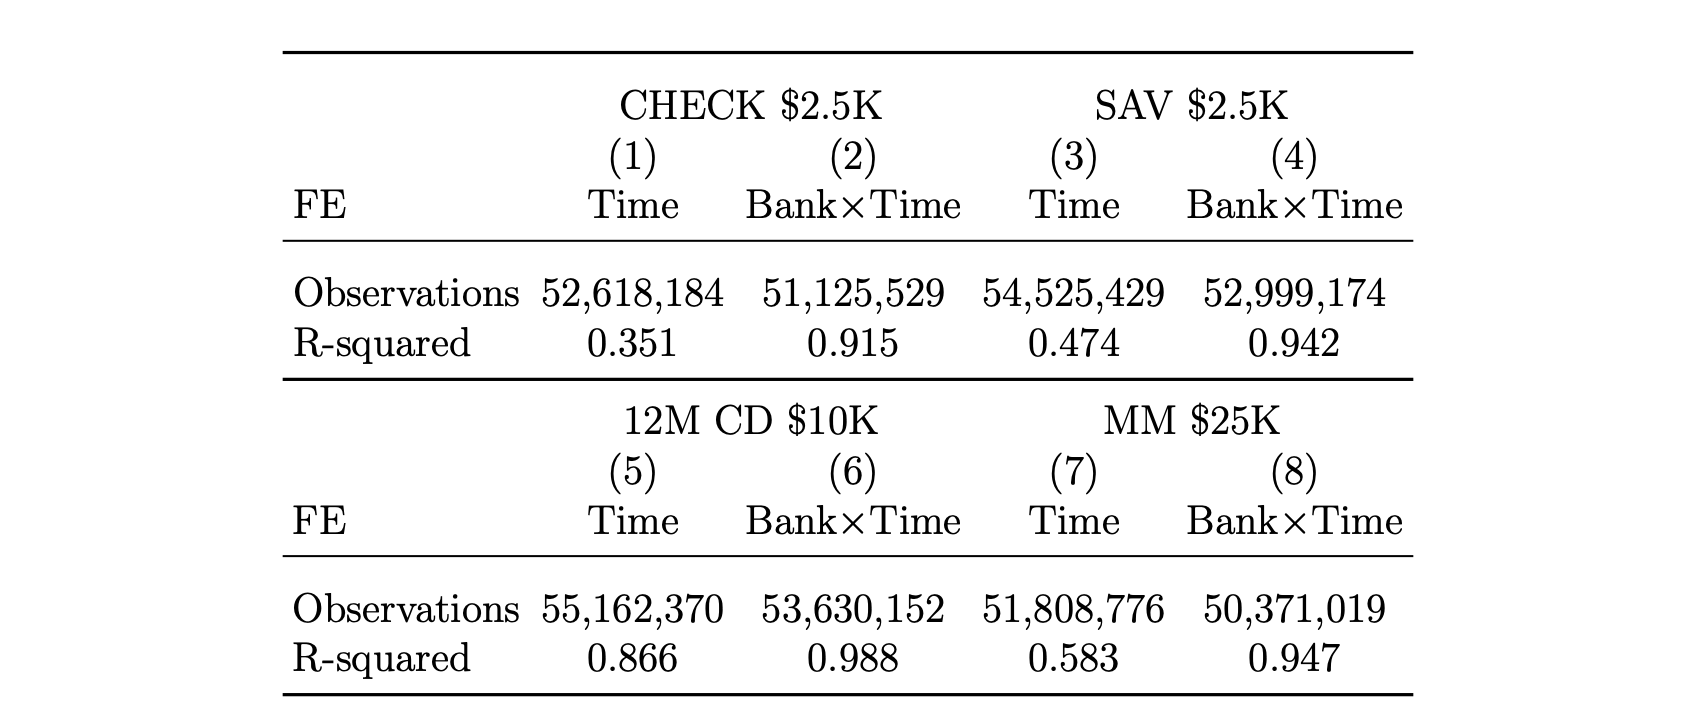
\includegraphics[width=0.69\textwidth]{imgs/tab1.png}
    \end{figure}

\end{frame}

\begin{frame}{Rate-setting behavior of large and small banks}

    \begin{columns}[T]
        
        \begin{column}{0.5\textwidth}
        
            \begin{figure}
                \centering
                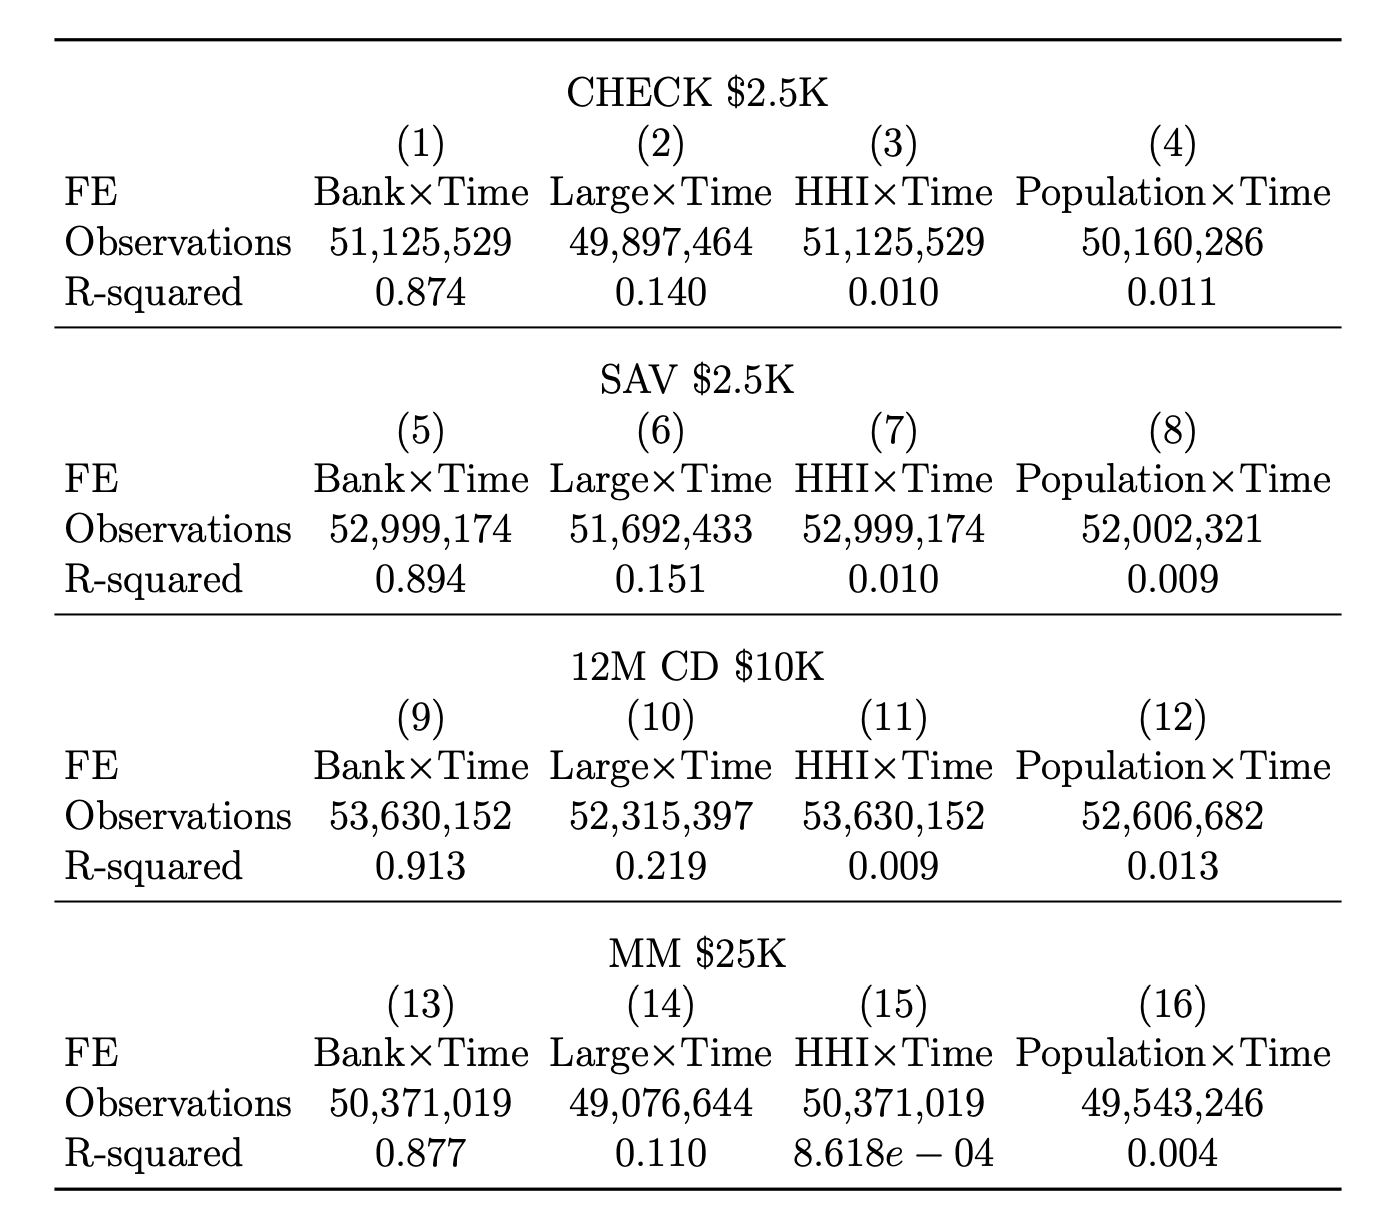
\includegraphics[width=0.95\textwidth]{imgs/tab2.png}
            \end{figure}

    \end{column}
    \begin{column}{0.5\textwidth}
        
        \begin{wideitemize}
            \item Two steps regressions, first time, then bank and market characteristics.
            \item Suggest bank and bank size, not market characteristics, drive rating.
        \end{wideitemize}
    \end{column}
    \end{columns}
    
\end{frame}

            
\begin{frame}{Smaller banks set higher rates than larger banks}


    \begin{figure}
        \centering
        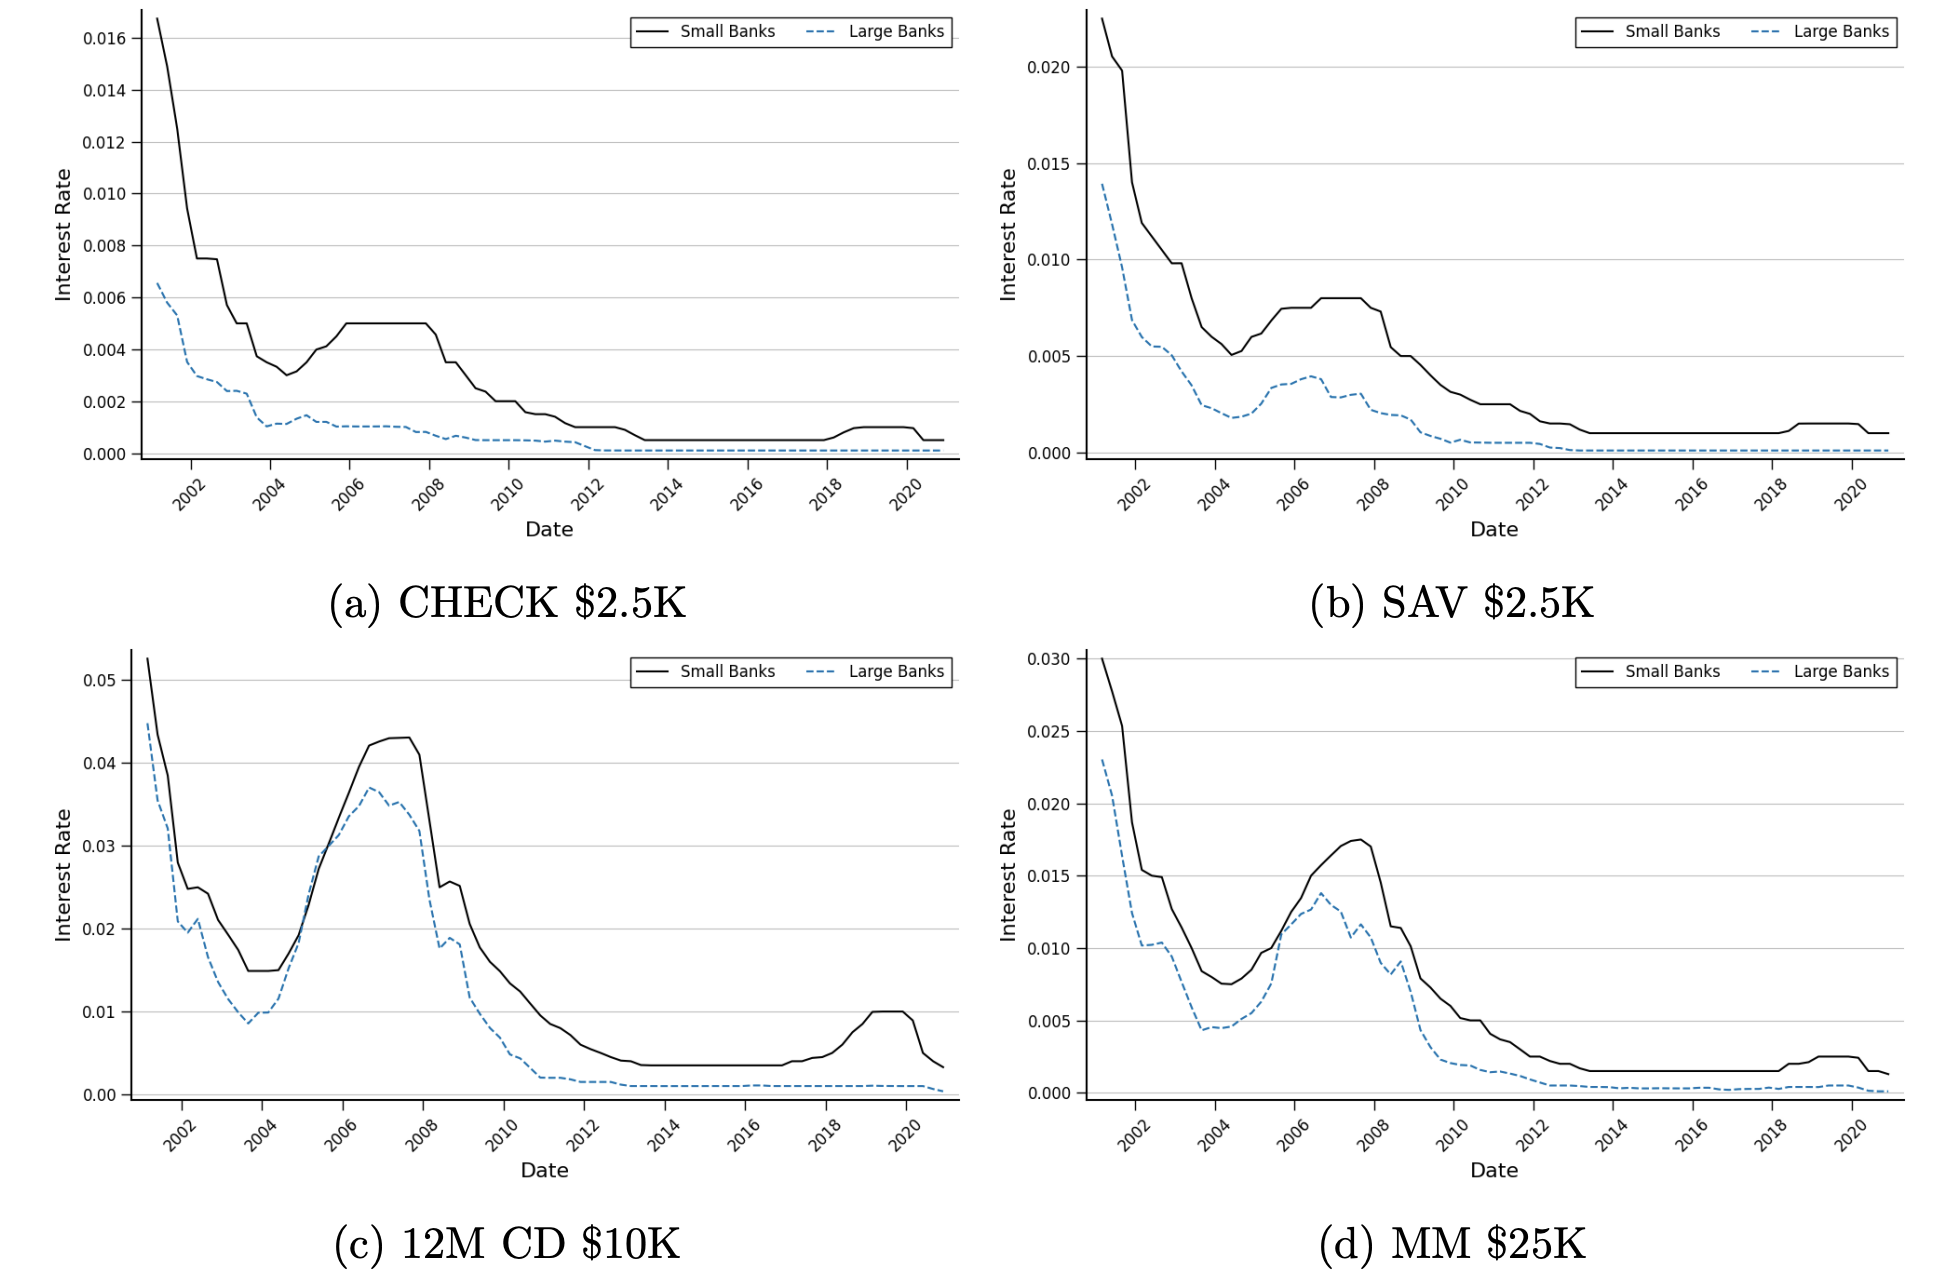
\includegraphics[width=0.76\textwidth]{imgs/fig1.png}
        % \caption*{ The use of wholesale funds across the bank size distribution in 1984.}
        % \label{fig:my_label}
    \end{figure}
    
\end{frame}

\begin{frame}{Smaller banks set higher rates than larger banks}

        % \begin{itemize}
        %     \item Banks close branches after adopting digital platforms.
        %     \item Expand service provision. 
        % \end{itemize}
    \begin{figure}
        \centering
        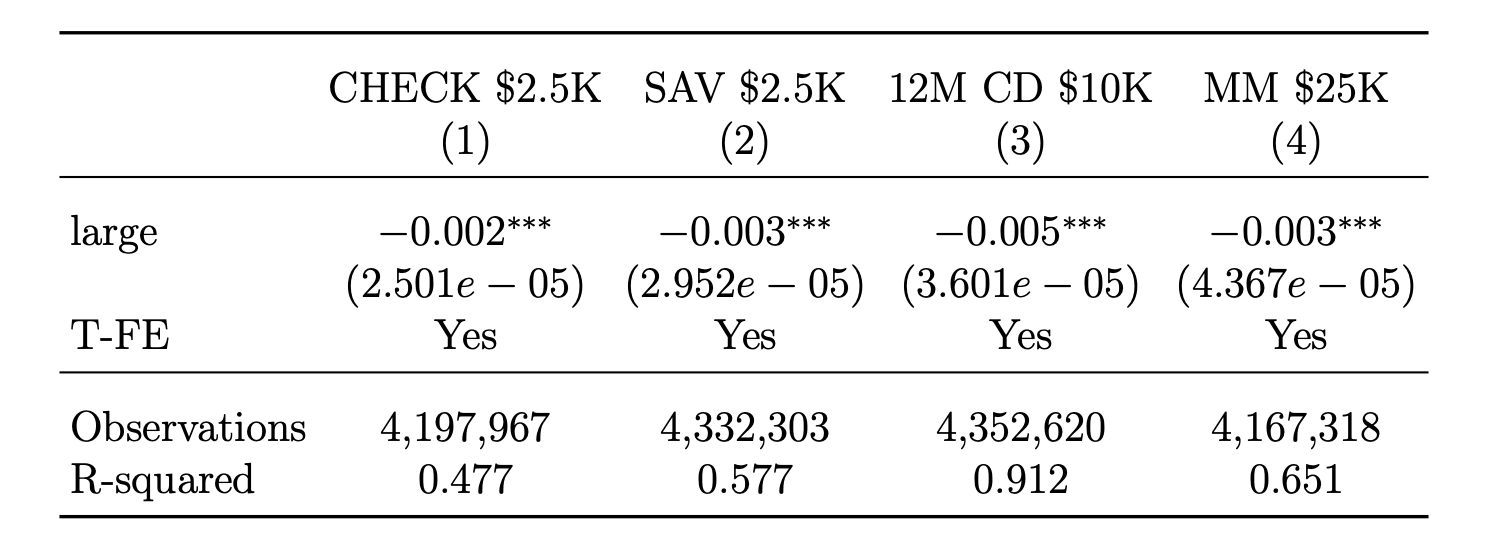
\includegraphics[width=0.65\textwidth]{imgs/tab3.png}
    \end{figure}

\end{frame}
    
    \begin{frame}{Deposit rates and market shares of large banks}

    
        \begin{figure}
            \centering
            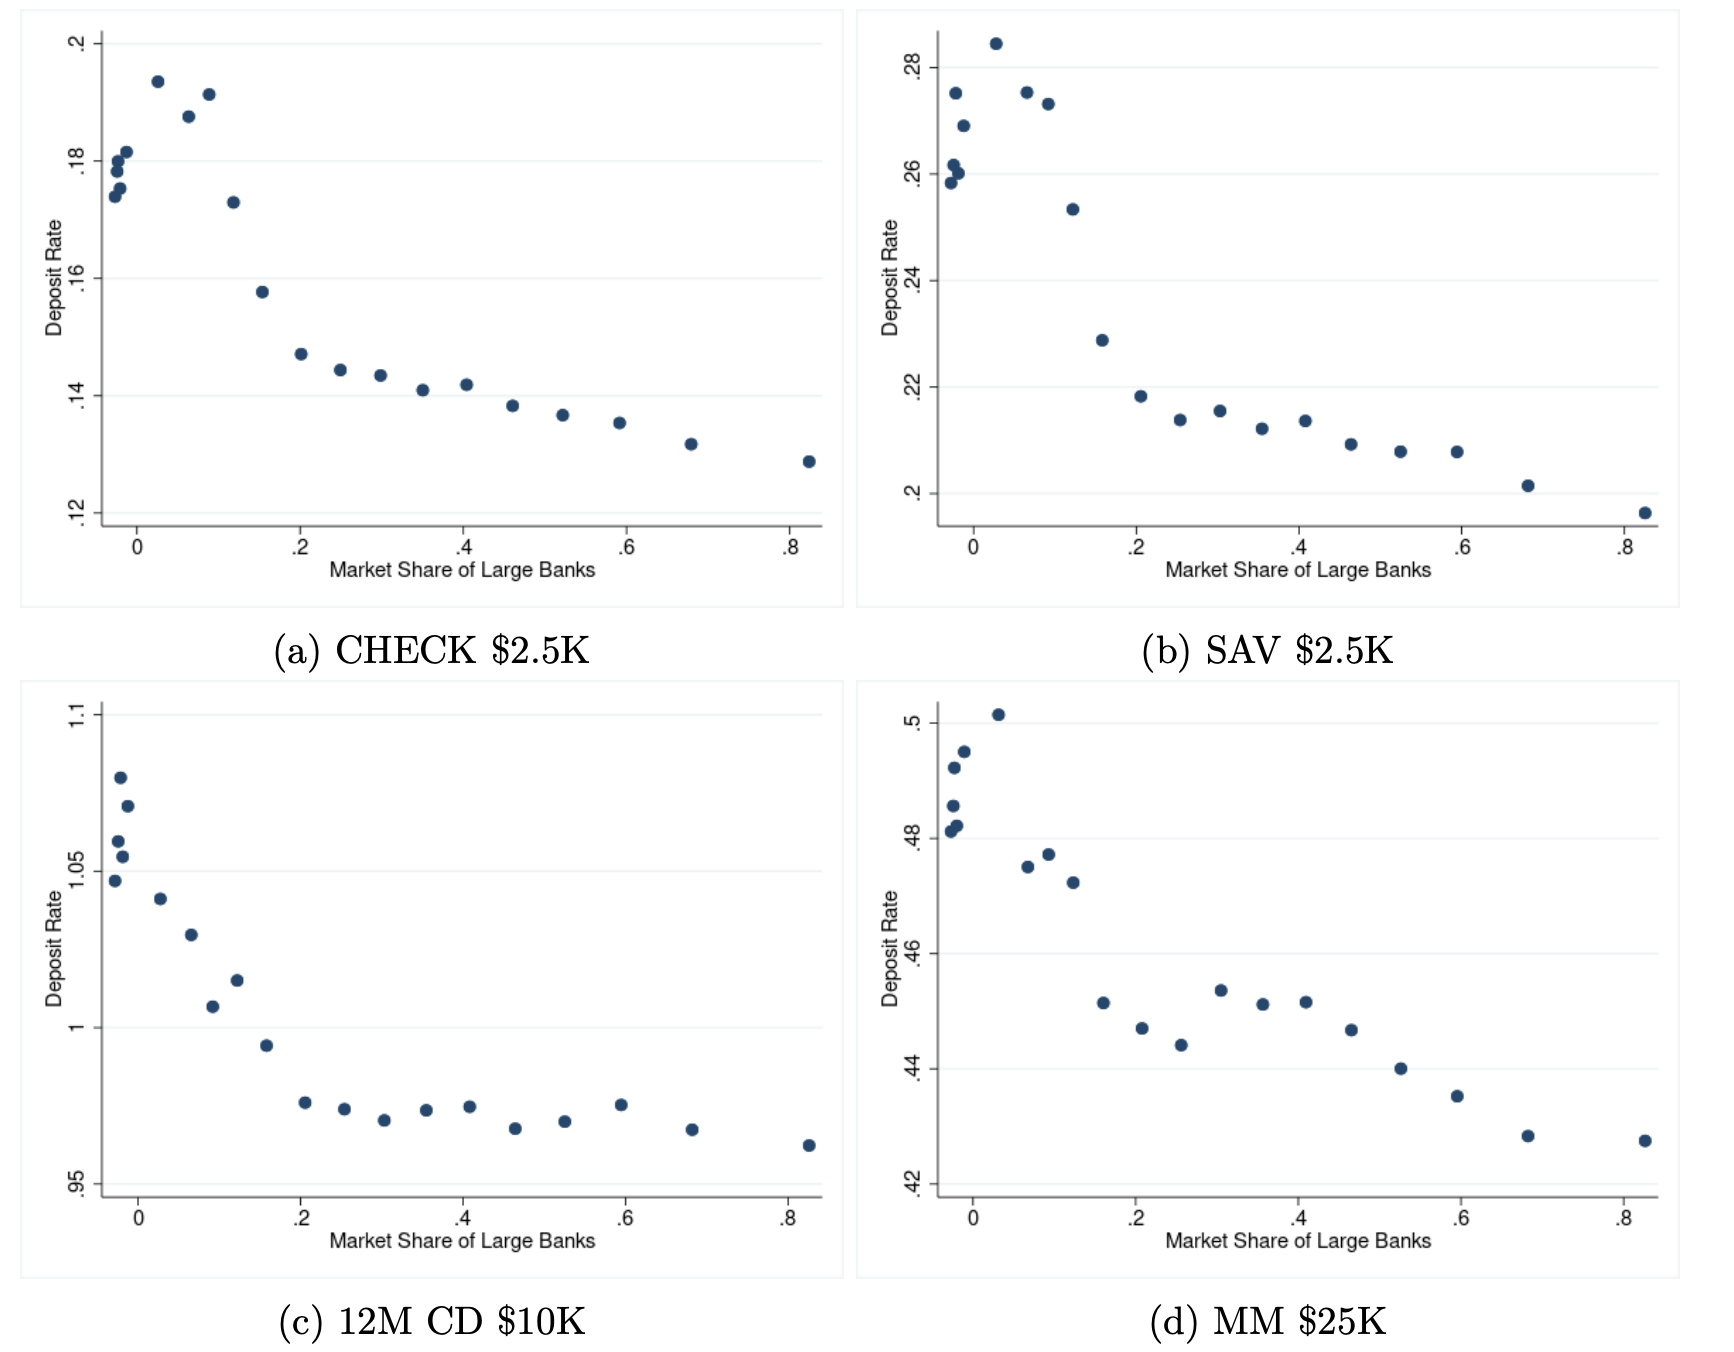
\includegraphics[width=0.7\textwidth]{imgs/fig2.png}
            % \caption*{ The use of wholesale funds across the bank size distribution in 1984.}
            % \label{fig:my_label}
        \end{figure}
        
    \end{frame}

% ********************************************************************************************************************
\begin{frame}{Large banks are concentrated in large markets}

    % \begin{wideitemize}
    
        \begin{wideitemize}
            %How did this expansion affect spatial sorting patterns? 
            \item bla bla
    \end{wideitemize}
    
    \begin{figure}
    \centering
    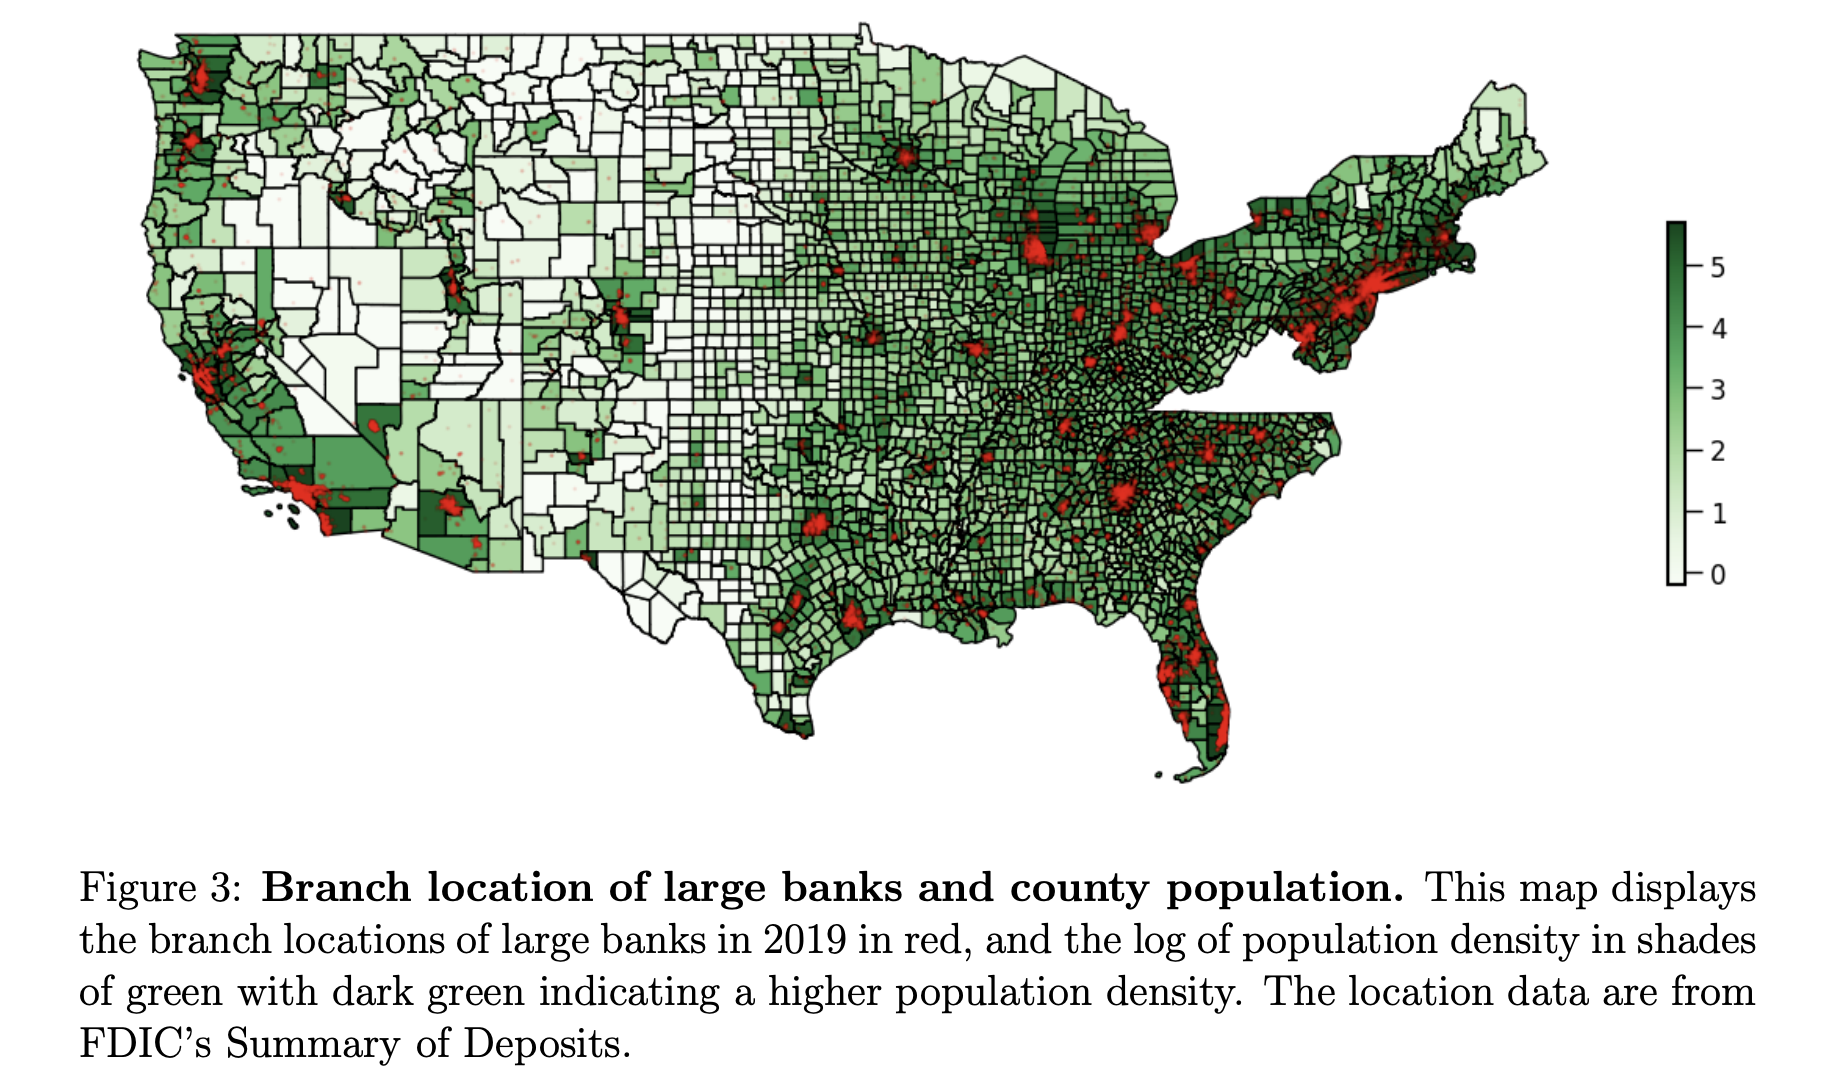
\includegraphics[width=0.8\textwidth]{imgs/fig3_foot.png}
    \end{figure}
    
    \end{frame}

\begin{frame}{Smaller banks have more branches in small markets}

    % \begin{wideitemize}
    
    %     \begin{wideitemize}
    %         %How did this expansion affect spatial sorting patterns? 
    %         \item bla bla
    % \end{wideitemize}
    
    \begin{figure}
    \centering
    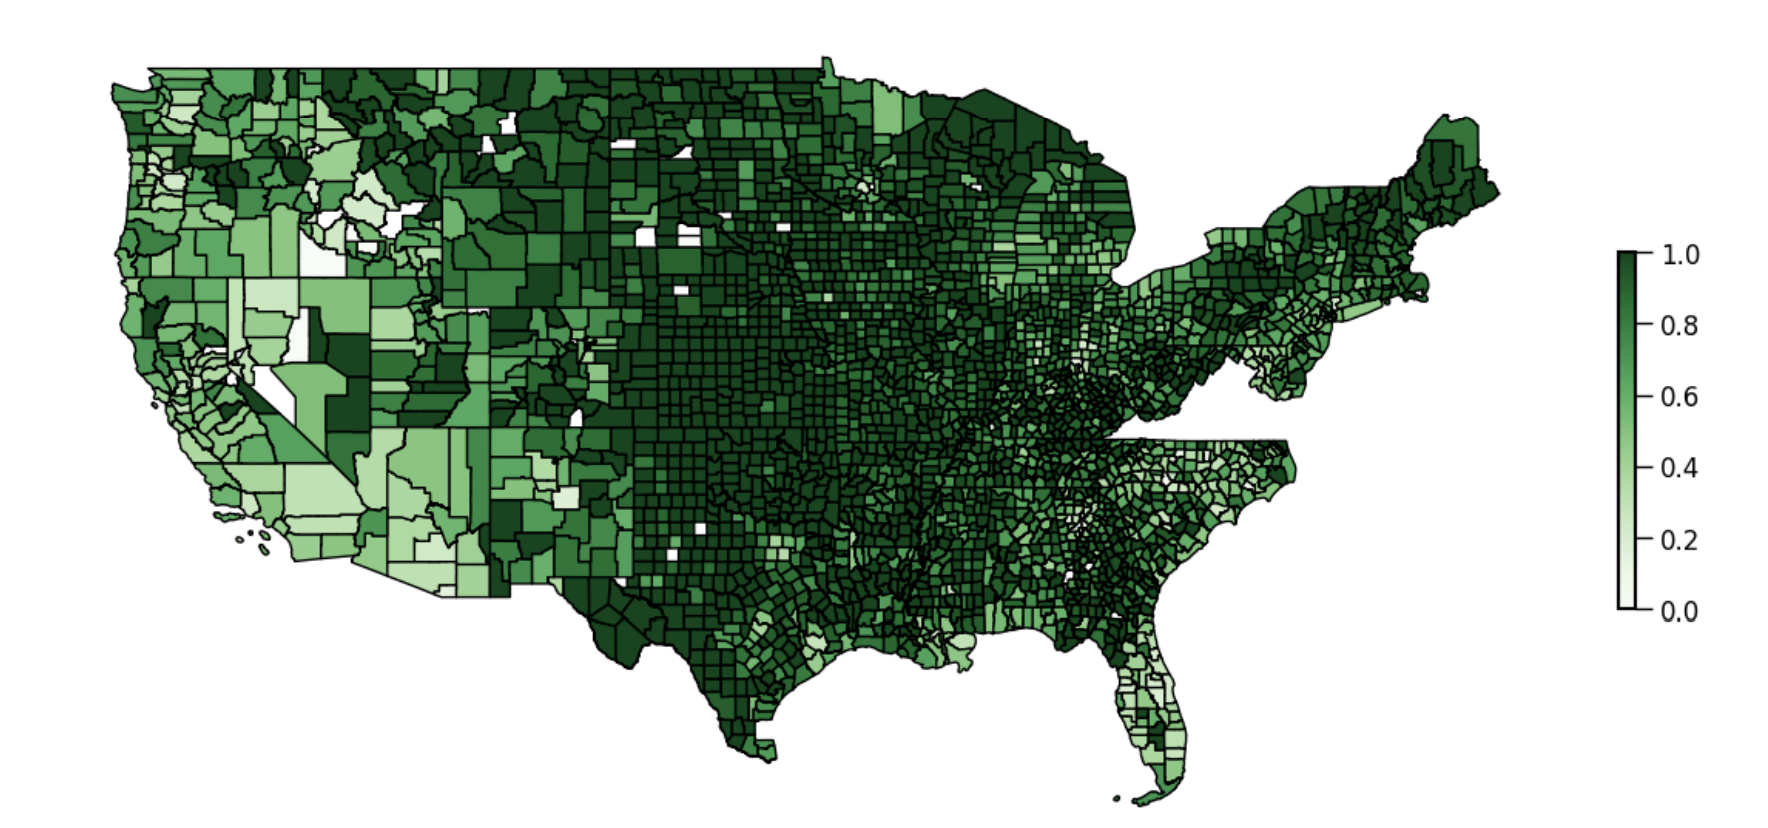
\includegraphics[width=0.8\textwidth]{imgs/fig4.png}
    %\caption*{Caption}
    % \label{fig:my_label}
    \end{figure}
    
    \end{frame}

\begin{frame}{Customer demographics}
    
        \begin{wideitemize}
            %How did this expansion affect spatial sorting patterns? 
            \item Small banks: less populated, more elderly, less income, and lower housing prices.
    \end{wideitemize}
    
    \begin{figure}
    \centering
    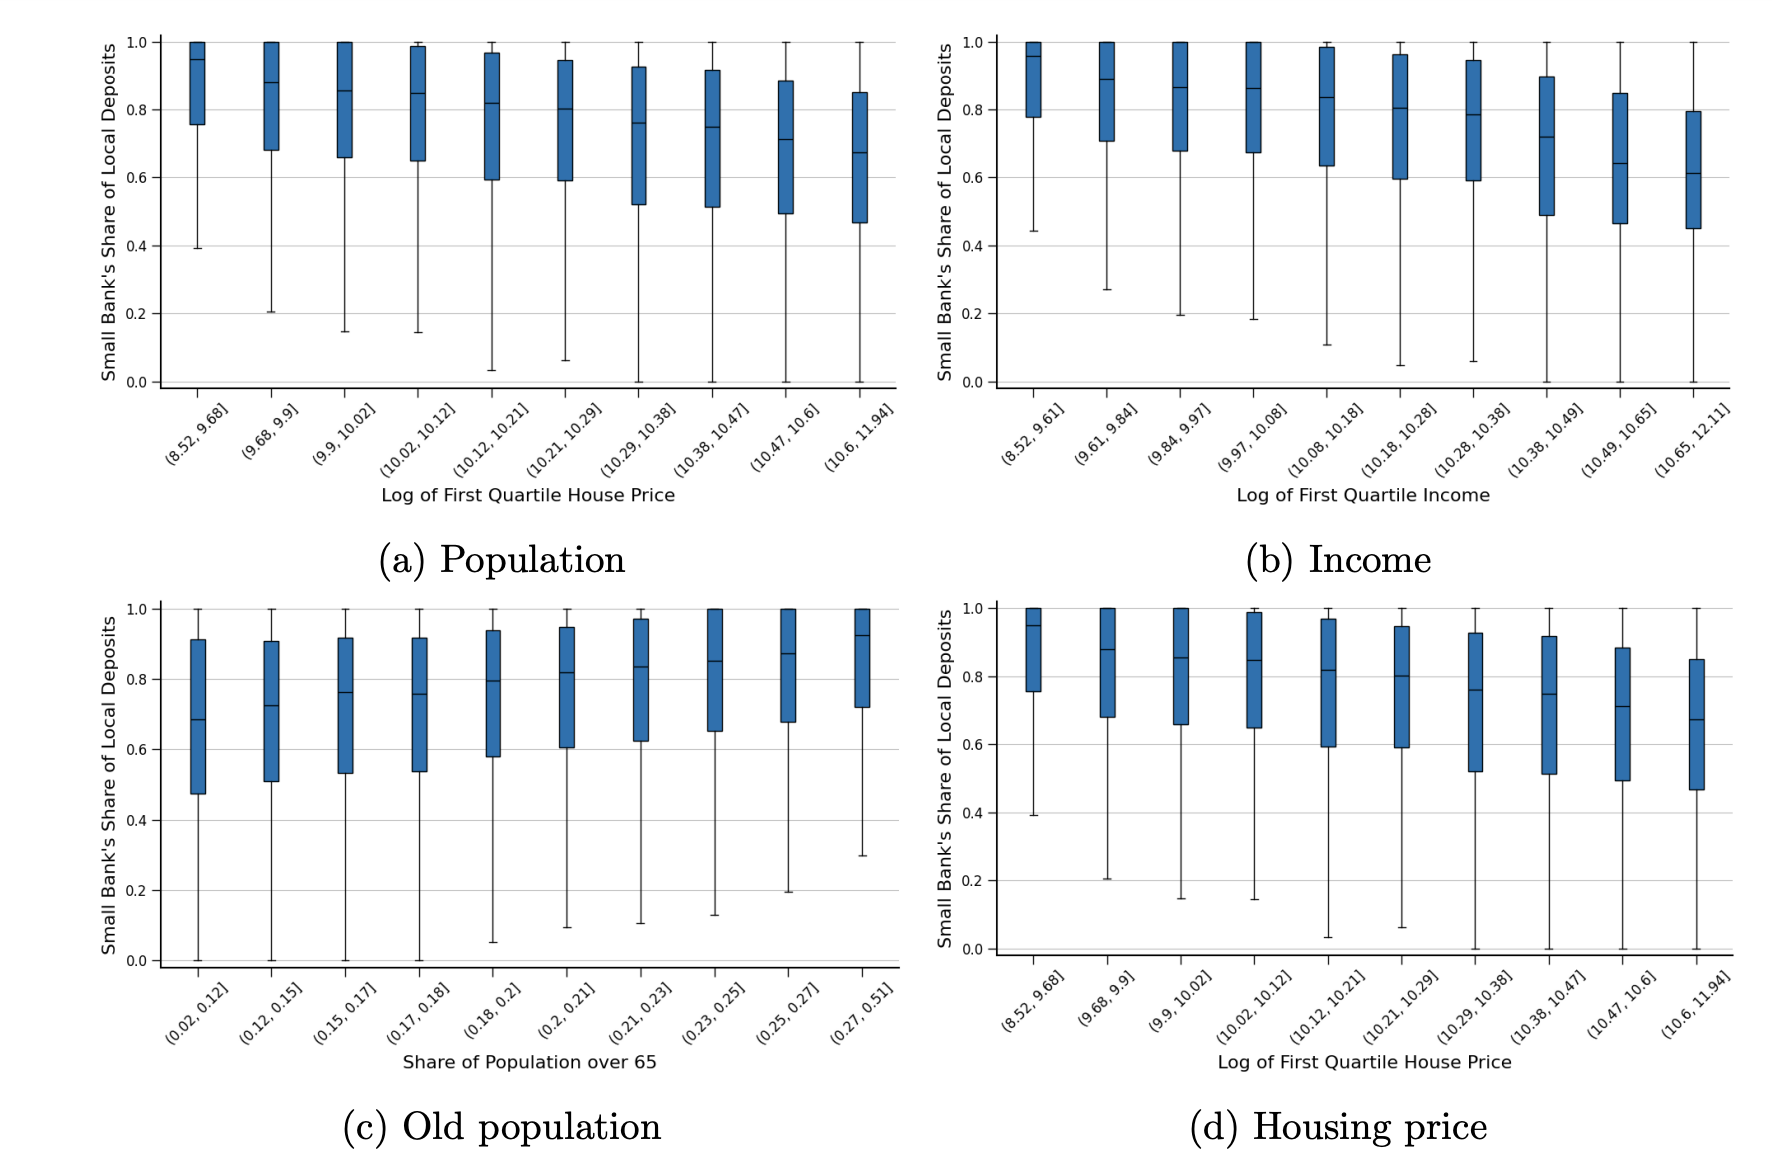
\includegraphics[width=0.8\textwidth]{imgs/fig5.png}
    %\caption*{Caption}
    % \label{fig:my_label}
    \end{figure}
    
    \end{frame}

    \begin{frame}{Customer demographics}

        % \begin{wideitemize}
        
            \begin{wideitemize}
                %How did this expansion affect spatial sorting patterns? 
        
                \item Small banks hold more liquid assets and agricultural loans.
                \item Large banks hold more saving deposits while small banks hold more time and transaction deposits.
        \end{wideitemize}
        
        \begin{figure}
        \centering
        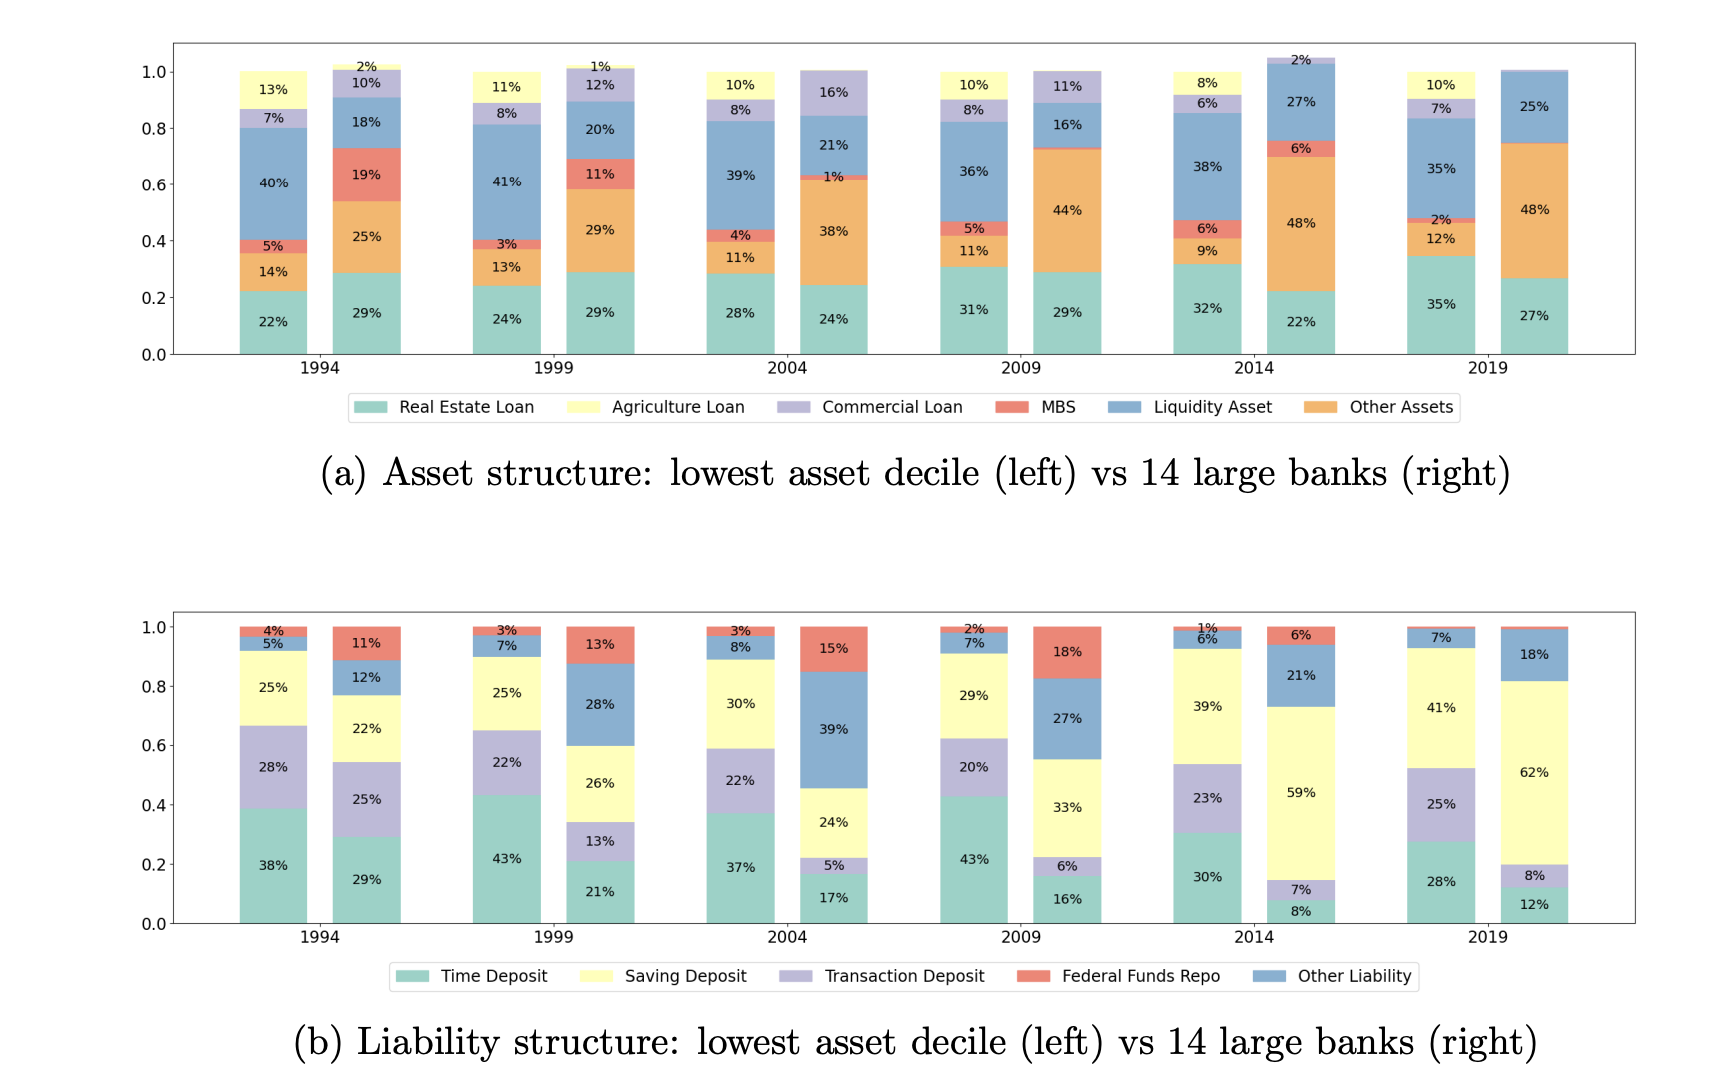
\includegraphics[width=0.7\textwidth]{imgs/fig7.png}
        %\caption*{Caption}
        % \label{fig:my_label}
        \end{figure}
        
        \end{frame}
    
    


% * Possible summary slide with evidence

% 5.3 Market selection conclusions
% In summary, the asset and liability structures of small and large banks are consistent with
% segmentation between their customer bases and with diferences in rate-setting behavior
% arising from variation in the production functions of large and small banks. We fnd that
% large banks typically operate in densely populated markets with higher household income,
% housing prices, and fewer elderly individuals and they hold more complex fnancial assets,
% consistent with technological diferences between large and small banks.
% \begin{frame}{Market selection conclusions}

% \vspace{0.1cm}


% %! Summary of the results
% \begin{wideitemize}
% \item The asset and liability structures of small and large banks are consistent with segmentation between their customer bases and with differences in rate-setting behavior arising from variation in the production functions of large and small banks.
% \item Large banks typically operate in densely populated markets with higher household income, housing prices, and fewer elderly individuals and they hold more complex financial assets, consistent with technological differences between large and small banks. 
% \end{wideitemize}
    
        
%         \end{frame}

% ********************************************************************************************************************


\begin{frame}[noframenumbering]

\huge \centering \textcolor{blue}{Estimation}

\end{frame}
    

        % * Nice slide with colored equations 


% $$
% U_{i, j, k, t}=-\alpha_i s_{j, k, t}+\beta X_{j, k, t}+\xi_{j, k, t}+\epsilon_{i, j, k, t}
% $$

% where $\xi_{j, k, t}=\xi_j+\xi_{k, t}+\Delta \xi_{j, k, t}$ consists of bank fixed effects $\xi_j$, market fixed effects $\xi_{k, t}$, and unobserved product characteristics $\Delta \xi_{j, k, t}$, where $\Delta \xi_{j, k, t}=\xi_{j, k, t}-\xi_j-\xi_{k, t}$. We allow customers to have heterogeneous rate sensitivity, represented by a normal distribution dependent on customer demographic $D_i$, i.e., $\alpha_i=\alpha+\Pi D_i+\sigma \nu_i$, where $\nu_i \sim N(0,1)$. The shock term $\epsilon_{i, j, k, t}$ is a stochastic term capturing customer-product specific shocks, which we assume follow a Type I extreme-value distribution with $F(x)=e^{-e^{-x}}$.






\begin{frame}{Estimation}

    % \begin{wideitemize}
        \vspace{0.3cm}
        \begin{wideitemize}
    
            \item Large banks are the 14 largest banks. 
            
            \item Bonds are the outside option
            % \begin{itemize}
            % \item Bonds are the outside option
            % \end{itemize}
            \item The utility specification is
            $$
            \begin{aligned}
            U_{i, j, k, t} & =-\alpha s_{j, k, t}-\left(\Pi D_i+\sigma \nu_i\right) s_{j, k, t}+\beta X_{j, k, t}+\xi_{j, k, t}+\epsilon_{i, j, k, t} \\
            & =\delta_{j, k, t}-\left(\Pi D_i+\sigma \nu_i\right) s_{j, k, t}+\epsilon_{i, j, k, t}
            \end{aligned}
            $$

    \begin{itemize}
        \item where $D_i$ is customer demographics, $\nu_i \sim N(0,1)$, and $\epsilon_{i, j, k, t}$ is a Type I EV.
    \end{itemize}
    \item The market share of product $j$ in a county cluster $k$ at time $t$ is

    $$
    \begin{aligned}
    d_{j, k, t}\left(X_{j, k, t}, s_{j, k, t} ; \alpha, \Pi, \beta, \sigma\right) & =\int\left(d_{i, j, k, t} d F_D(D) d F_\nu(\nu)\right. \\
    & =\frac{1}{N} \sum_{i=1}^N \frac{\exp \left(\delta_{j, k, t}+\left(\Pi D_i+\sigma \nu_i\right) s_{j, k, t}\right)}{1+\sum_{l=1}^{J+1} \exp \left(\delta_{l, k, t}+\left(\Pi D_i+\sigma \nu_i\right) s_{l, k, t}\right)},
    \end{aligned}
    $$
    
    \end{wideitemize}

\end{frame}



\begin{frame}{Instruments and Identification Argument}
    \begin{wideitemize}
        % \item \textbf{Challenge:} Endogeneity in deposit rates (\(r_{j,k,t}\)) leads to biased estimates.  
        \item \textcolor{blue}{Solution:} Use supply shocks (\(Z_{j,k,t}\)) as instruments:  
        \begin{itemize}
            \item Staff salaries to total assets (prior year).  
            \item Non-interest expenses to total assets (prior year).  
            \item Local labor costs (county-level, weighted by deposits).  
        \end{itemize}
        \item \textcolor{blue}{Assumption:} Customers do not respond to cost changes, but banks adjust rates.  
        \item \textcolor{blue}{Estimation:} IV-GMM following BLP (1995).  
    \end{wideitemize}
\end{frame}


\begin{frame}{Summary Statistics}
    % \begin{wideitemize}
    %     \item 
    % \end{wideitemize}

    \begin{figure}
    \centering
    \begin{minipage}{0.9\textwidth}
%  {\footnotesize
%  Controls include establishments, employment, payroll, deposit, loan growth, and year fixed effects.}
        \end{minipage}
    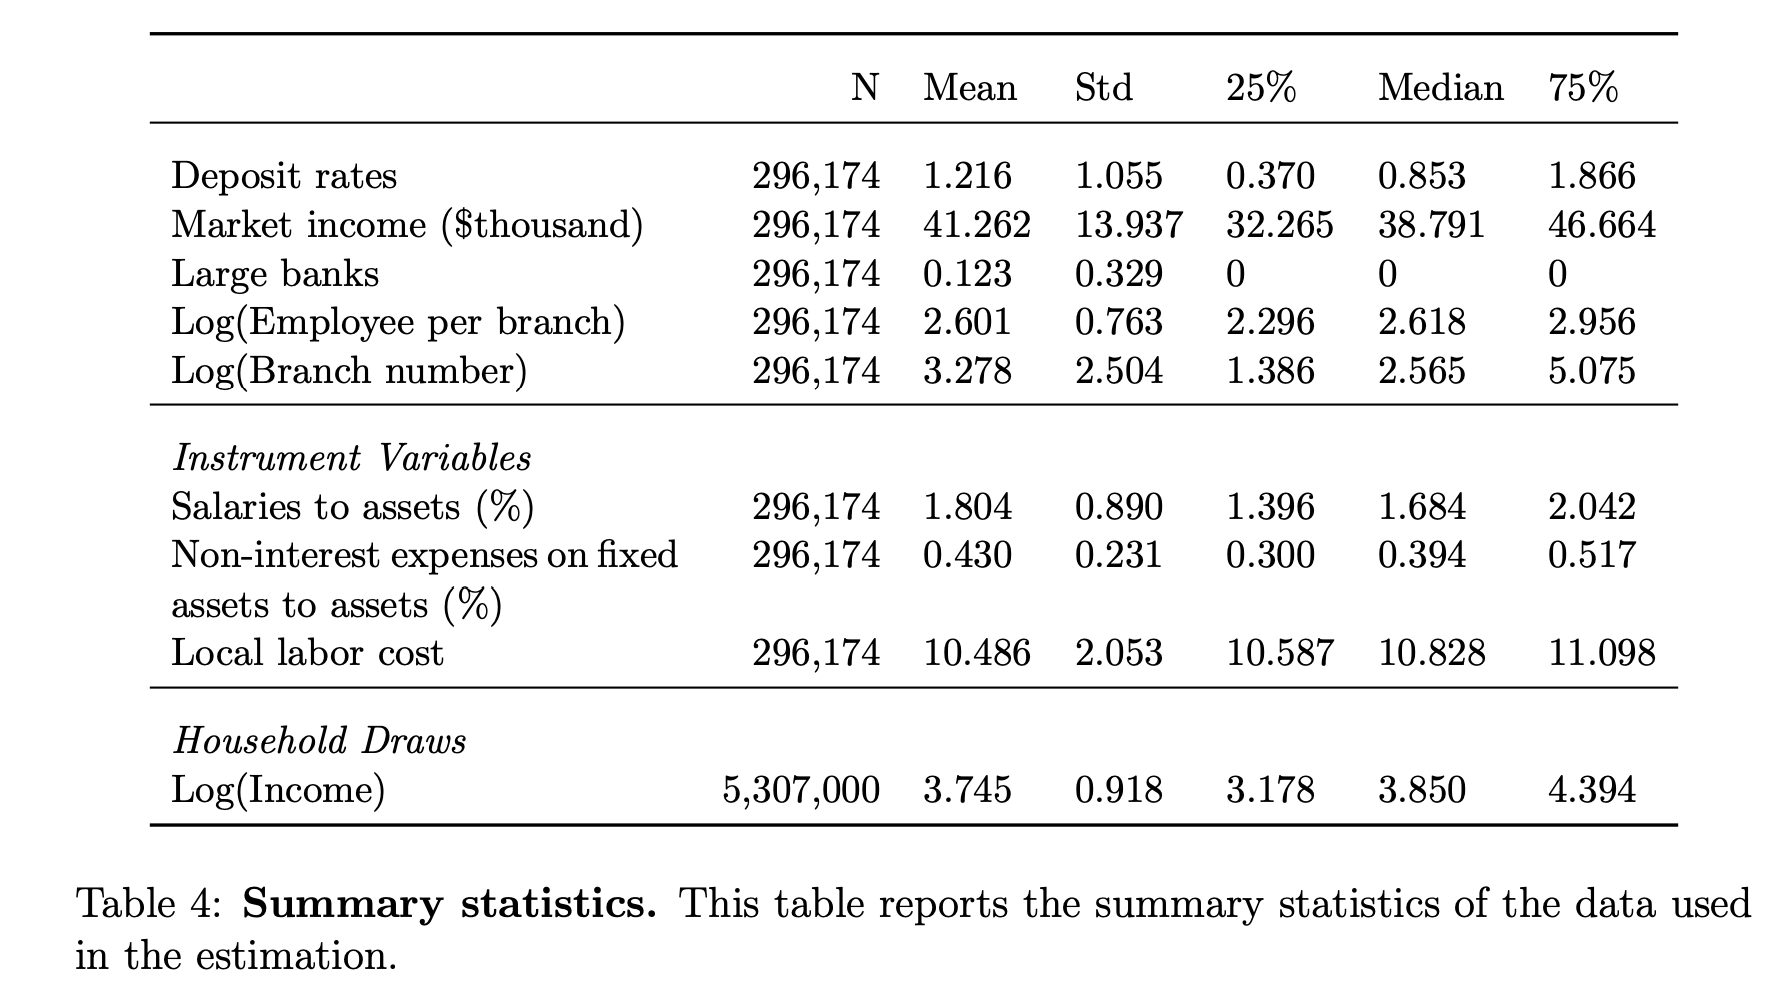
\includegraphics[width=0.85\textwidth]{imgs/tab4.png}
    \end{figure}
\end{frame}





% \begin{frame}{Corporate deposits are flowing to banks with digital platforms}
%     % \begin{itemize}
%     %     % \item conclusions of table here
%     % \end{itemize}

%     \begin{figure}
%     \centering
%     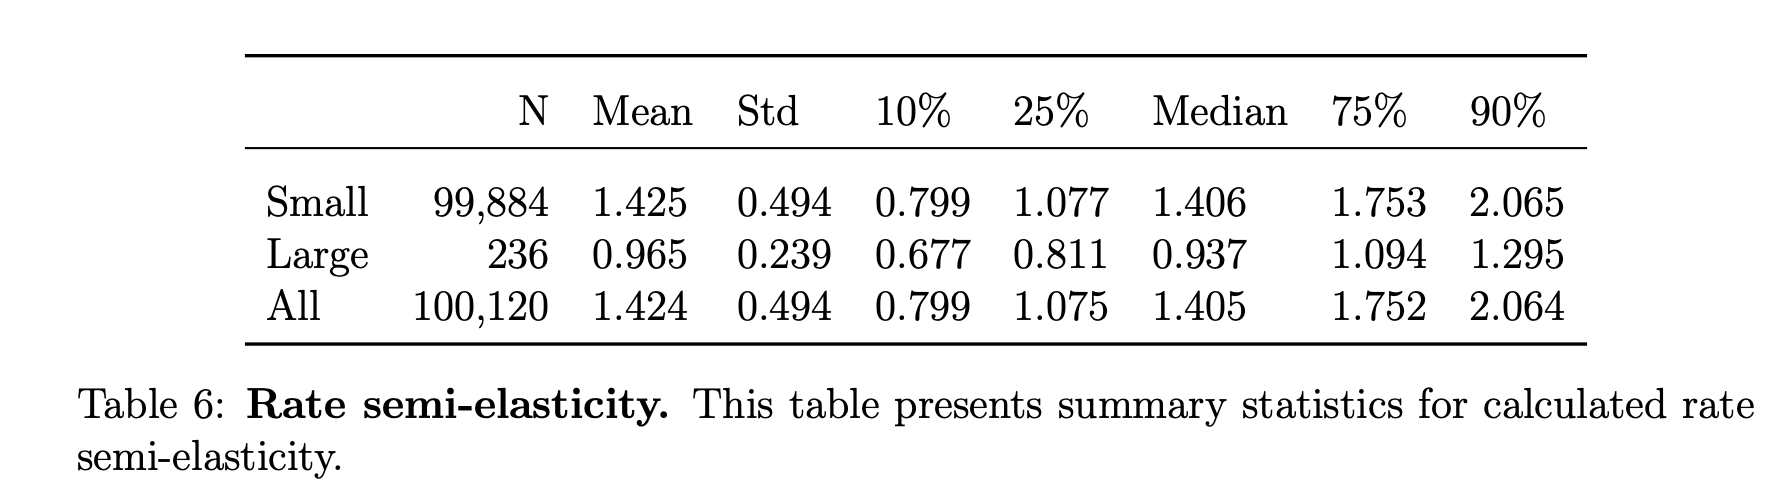
\includegraphics[width=0.7\textwidth]{imgs/tab6.png}
%     %\caption*{Caption}
%     % \label{fig:my_label}
%     % \caption*{Standard errors are two-way clustered at the state and bank level.}
%     \end{figure}

% \end{frame}


\begin{frame}{Rate semi-elasticities}

    \begin{itemize}
    \item Bank expansion into new counties driven by high-income borrowers.
    \end{itemize}
        \begin{figure}
            \centering
            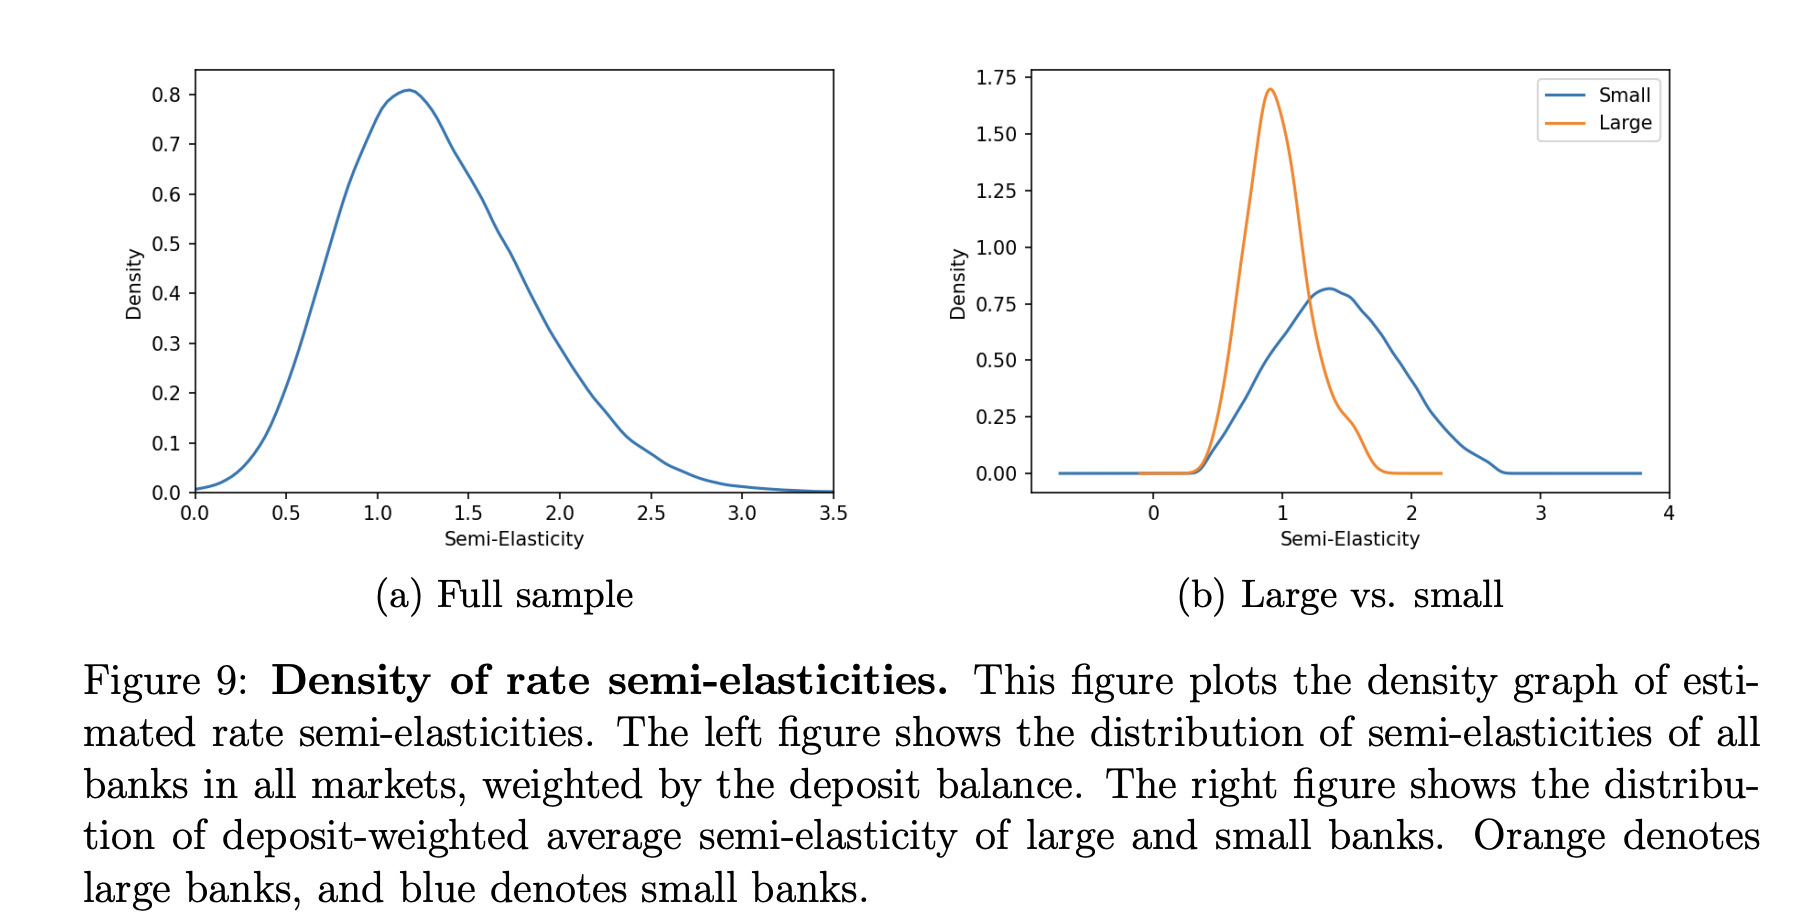
\includegraphics[width=0.7\textwidth]{imgs/fig9_foot.png}
            %\caption*{Caption}
            % \label{fig:my_label}
        \end{figure}
        
    \end{frame}
    
    

    \begin{frame}{Rate semi-elasticities and market shares}

    \begin{itemize}
    \item Bank expansion into new counties driven by high-income borrowers.
    \end{itemize}
        \begin{figure}
            \centering
            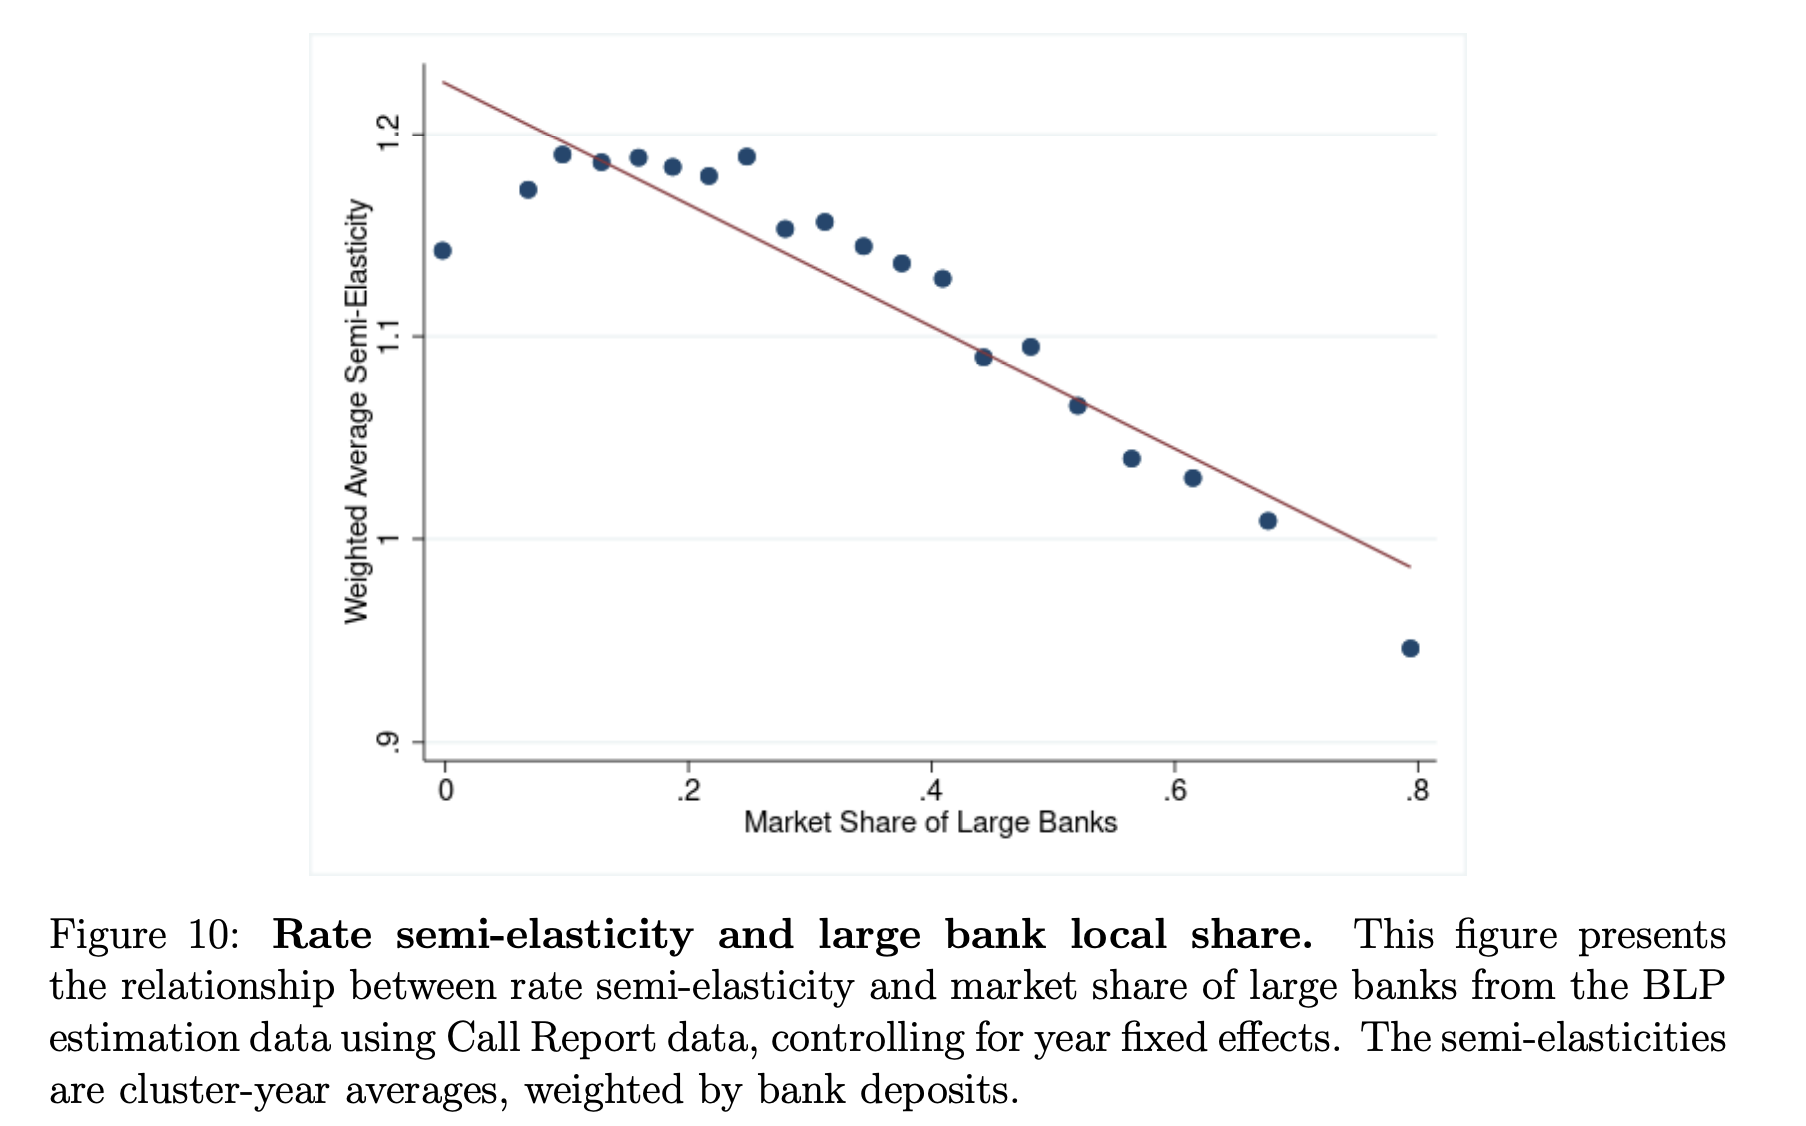
\includegraphics[width=0.65\textwidth]{imgs/fig10.png}
            %\caption*{Caption}
            % \label{fig:my_label}
        \end{figure}
        
\end{frame}


\begin{frame}{Rate semi-elasticities analysis}

    \begin{columns}[T]
        
        \begin{column}{0.5\textwidth}
        
            \begin{figure}
                \centering
                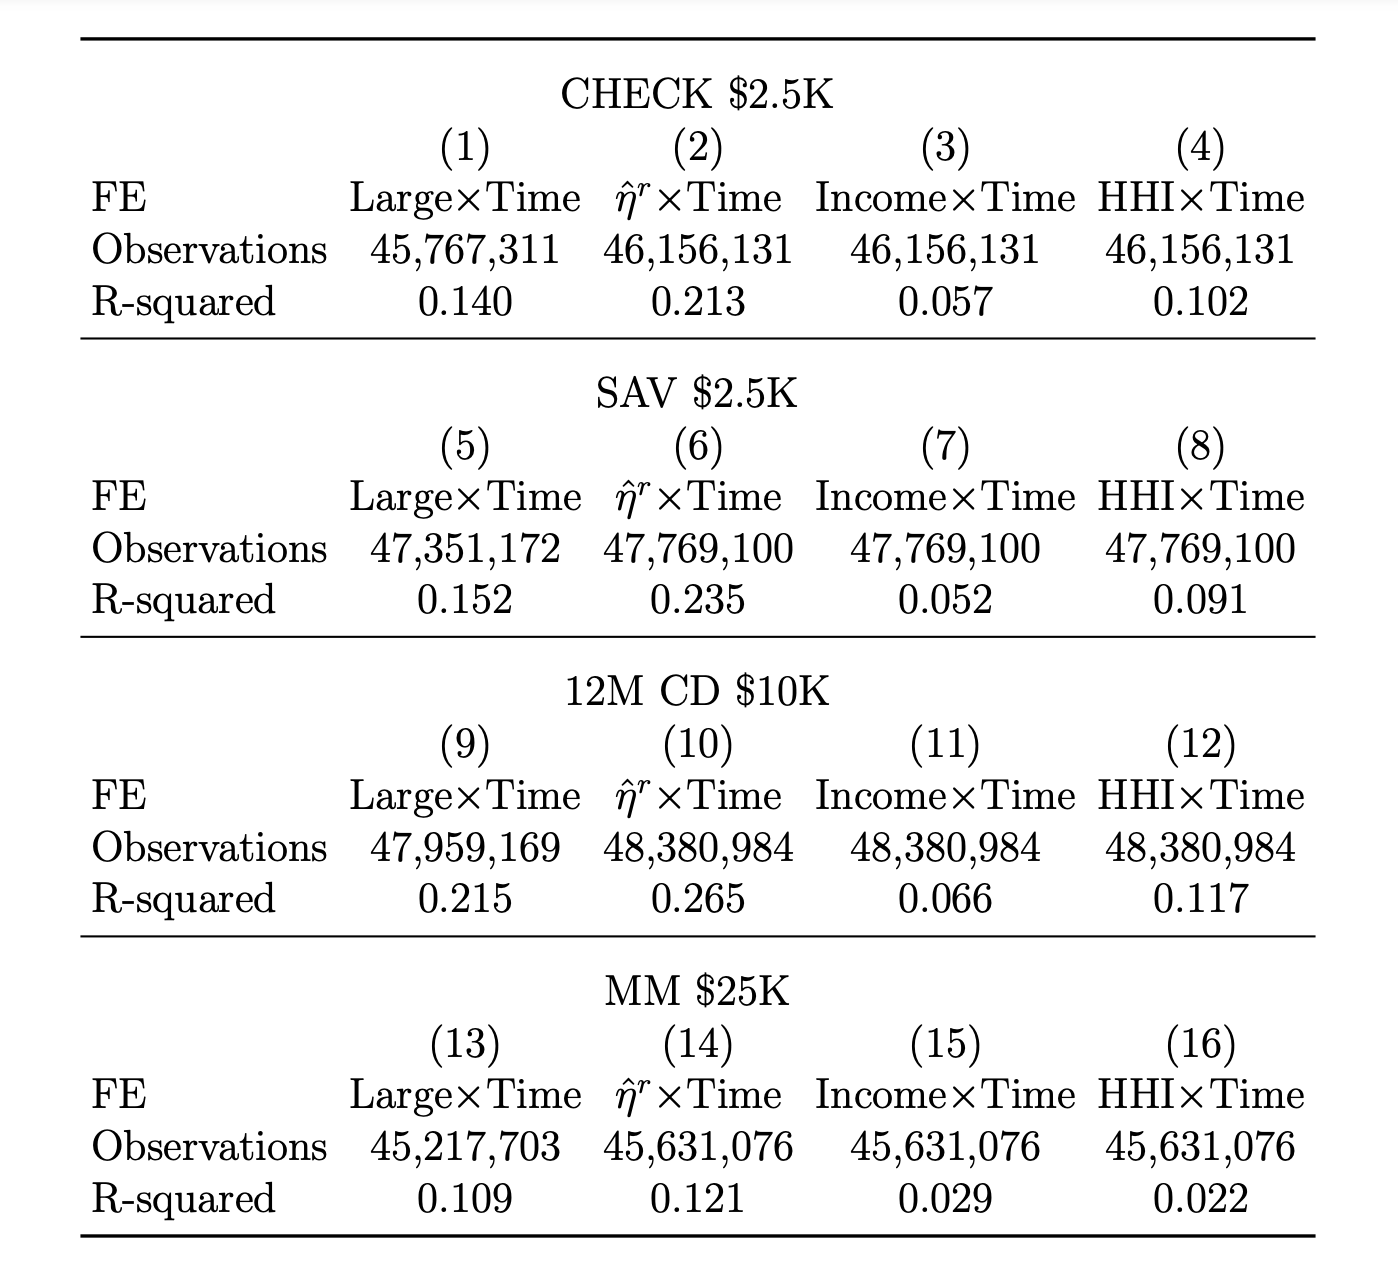
\includegraphics[width=0.95\textwidth]{imgs/tab7.png}
            \end{figure}

        \end{column}
        \begin{column}{0.5\textwidth}
        

            \begin{wideitemize}
                \item  Similar residual analysis with two-stage.
                \item The semielasticity-time FE accounts for between 12 \% and 26.5\% of the variation in deposit rates.
                % \item This is higher than the time FE alone.
            \end{wideitemize}
        \end{column}
    \end{columns}
            
\end{frame}
        
% Conclusion frame


\begin{frame}{Conclusions}
    \begin{wideitemize}
        \item Deposit rate setting reflects differences in \text{customer preferences} and \text{bank technologies}, not just market power.  
        \item Large banks' concentration may arise from \text{fixed costs of superior financial-service technologies} (e.g., ATMs, software).  
        \item Variations in deposit pricing highlight \text{heterogeneous production functions} for deposit franchises.  
    \end{wideitemize}
\end{frame}

    

    \begin{frame}{}
        % Thank you slide
        \centering
        \huge \textcolor{blue}{Thank you!}
    \end{frame}


    


\end{document}